\section{Funções de Engenharia}

Para cada função existente no projeto, as entradas, saídas e definições de retorno são descritas a seguir. Algumas rotinas recuperam informações do banco de dados local ou das bibliotecas utilizadas, enquanto outras calculam diretamente parâmetros de projeto.

\subsection{Dimensionamento de Tubulações}

Tubulações são componentes por onde o fluido escoa, permitindo a transferência de matéria entre equipamentos, desde a entrada de matéria-prima até a saída de produtos. Seu correto dimensionamento é imprescindível para a segurança e a eficiência do processo.

O dimensionamento consiste em definir o diâmetro nominal e o \textit{schedule} capazes de conduzir as vazões dentro de faixas de velocidade e perda de carga economicamente ótimas. As grandezas envolvidas incluem vazão (mássica ou volumétrica), velocidade admissível, propriedades do fluido (massa específica, viscosidade), comprimento equivalente (devido a acessórios) e características do material (rugosidade, pressão de projeto).

Na prática, calcula-se um diâmetro a partir da vazão e velocidade alvo e seleciona-se o diâmetro comercial imediatamente superior disponível, verificando em seguida a perda de carga pelo método de Darcy–Weisbach e a integridade mecânica conforme normas aplicáveis. Temperatura e pressão afetam propriedades físicas do fluido e critérios de espessura da tubulação; adicionalmente, a topografia da planta e o número de acessórios elevam o comprimento equivalente total.

Subdimensionar uma tubulação implica grandes perdas de carga e custos energéticos; superdimensionar acarreta CAPEX elevado e pode gerar velocidades muito baixas (favorecendo sedimentação em tubulações com sólidos). O embasamento teórico combina a equação de continuidade, correlações de atrito e seleção de materiais, apoiado no uso do diagrama de Moody \cite{white2018}.

\subsubsection{Diâmetro Calculado}

O diâmetro calculado é baseado na vazão e na velocidade média do fluido escoando em um duto circular, de acordo com a Equação \ref{eq:diametro_calc}:

\begin{equation}
D = \sqrt{\frac{4 \cdot Q}{\pi \cdot V}}
\label{eq:diametro_calc}
\end{equation}

Em que:
\begin{itemize}
    \item $Q$ -- vazão volumétrica do fluido;
    \item $V$ -- velocidade média do fluido;
    \item $D$ -- diâmetro hidráulico do duto circular.
\end{itemize}

Essa relação advém diretamente da equação da continuidade para escoamento em regime permanente \cite{white2018}. $Q$ em $\mathrm{m^3/s}$ e $V$ em $\mathrm{m/s}$ dão $D$ em $\mathrm{m}$ na equação; a rotina implementada converte o resultado exibido para $\mathrm{mm}$.

\begin{figure}[H]
    \centering
    \caption{Código da função \textit{get\_calculated\_diameter()}}
    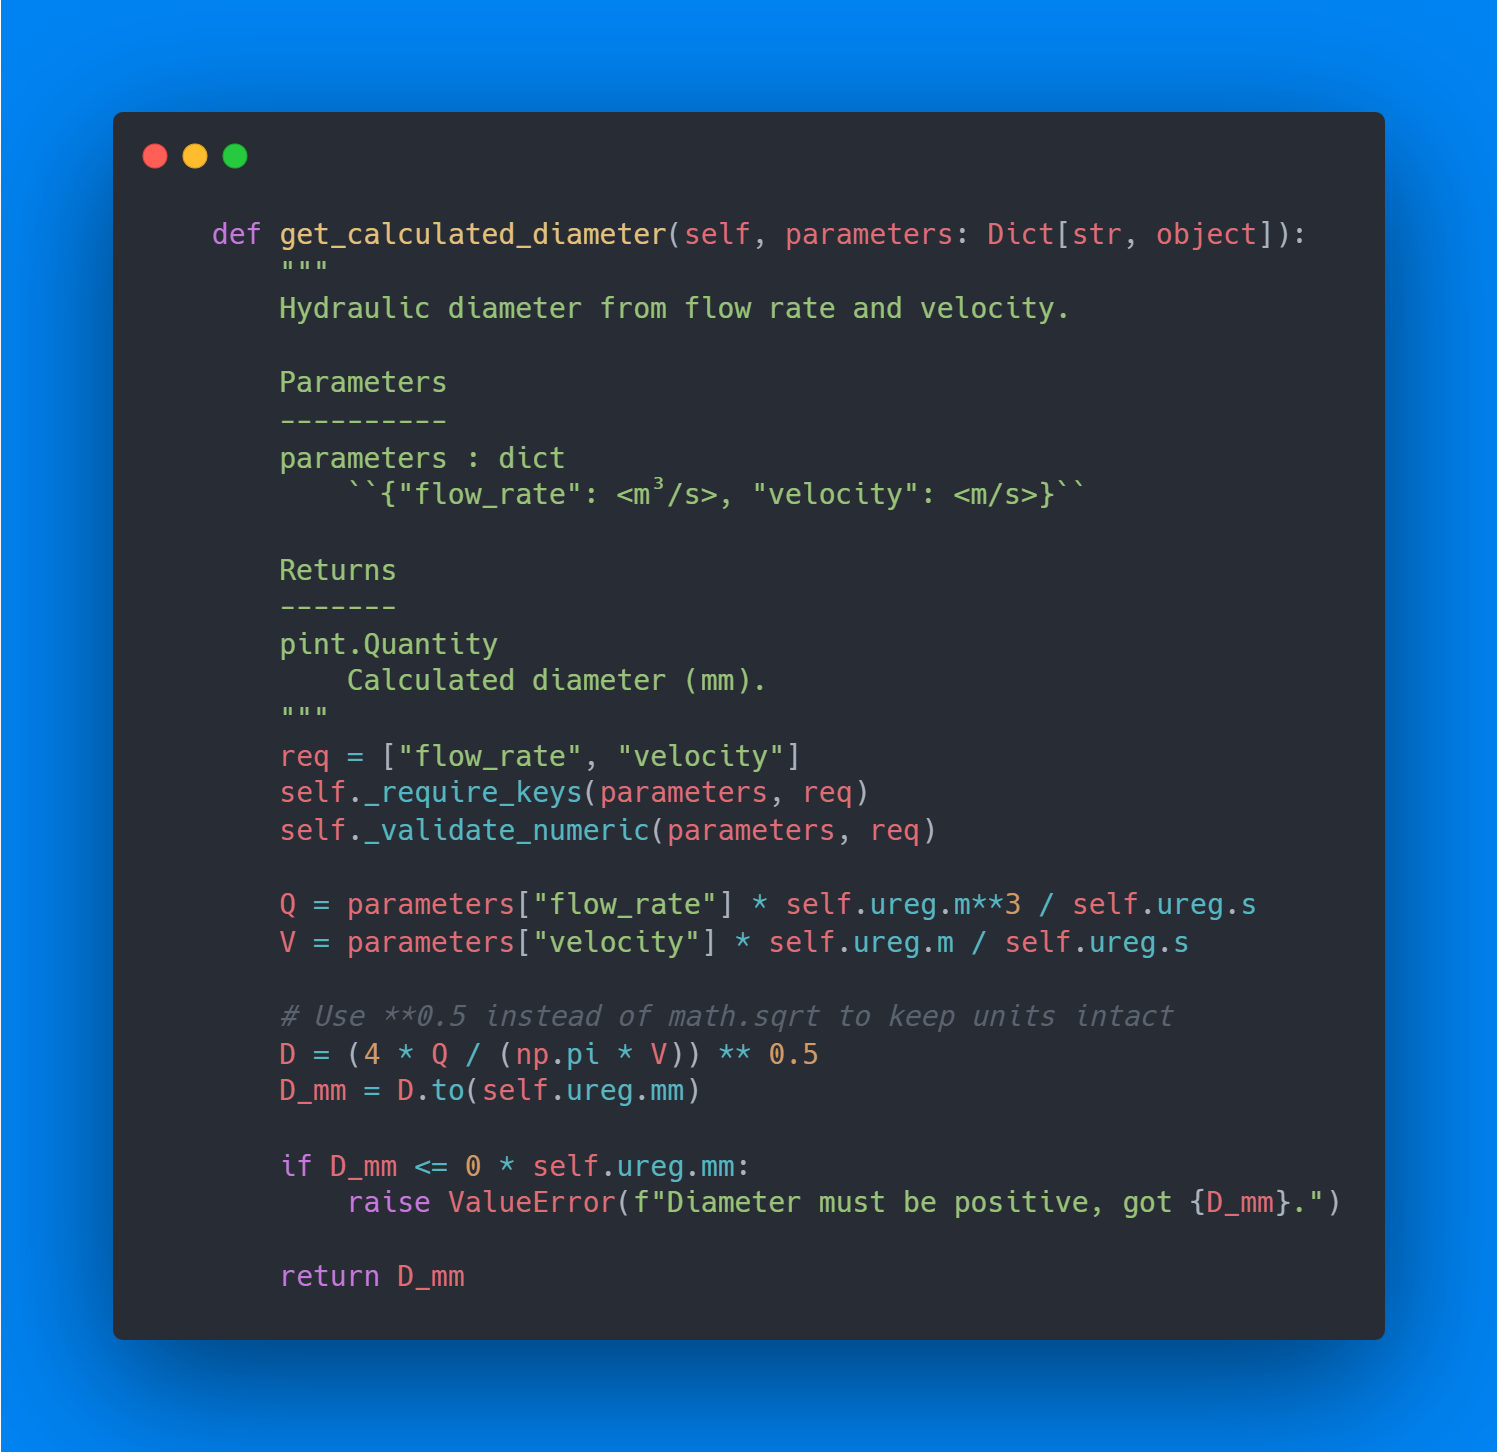
\includegraphics[width=\linewidth]{media/cap4_funcao_get_calculated_diameter.png}
    \fonte{Elaboração própria (2026).}
\end{figure}

\subsubsection{Diâmetro Real}

O diâmetro real corresponde ao diâmetro nominal da tubulação a ser utilizada. Fabricantes produzem tubos em geometrias padronizadas (padrões de espessura como SCH 10, SCH 40, SCH 80 etc.). Deve-se calcular inicialmente o diâmetro necessário pelo método anterior e então escolher, em tabela de catálogo, o tubo comercial com diâmetro interno imediatamente superior, no material e \textit{schedule} desejados. Essa lógica é implementada na função \textit{get\_real\_diameter}, garantindo que o diâmetro selecionado comportará a vazão com velocidade dentro do admissível. Após a seleção, verifica-se a perda de carga resultante e, se necessário, itera-se para outro diâmetro.

\begin{figure}[H]
    \centering
    \caption{Código da função \textit{get\_real\_diameter()}}
    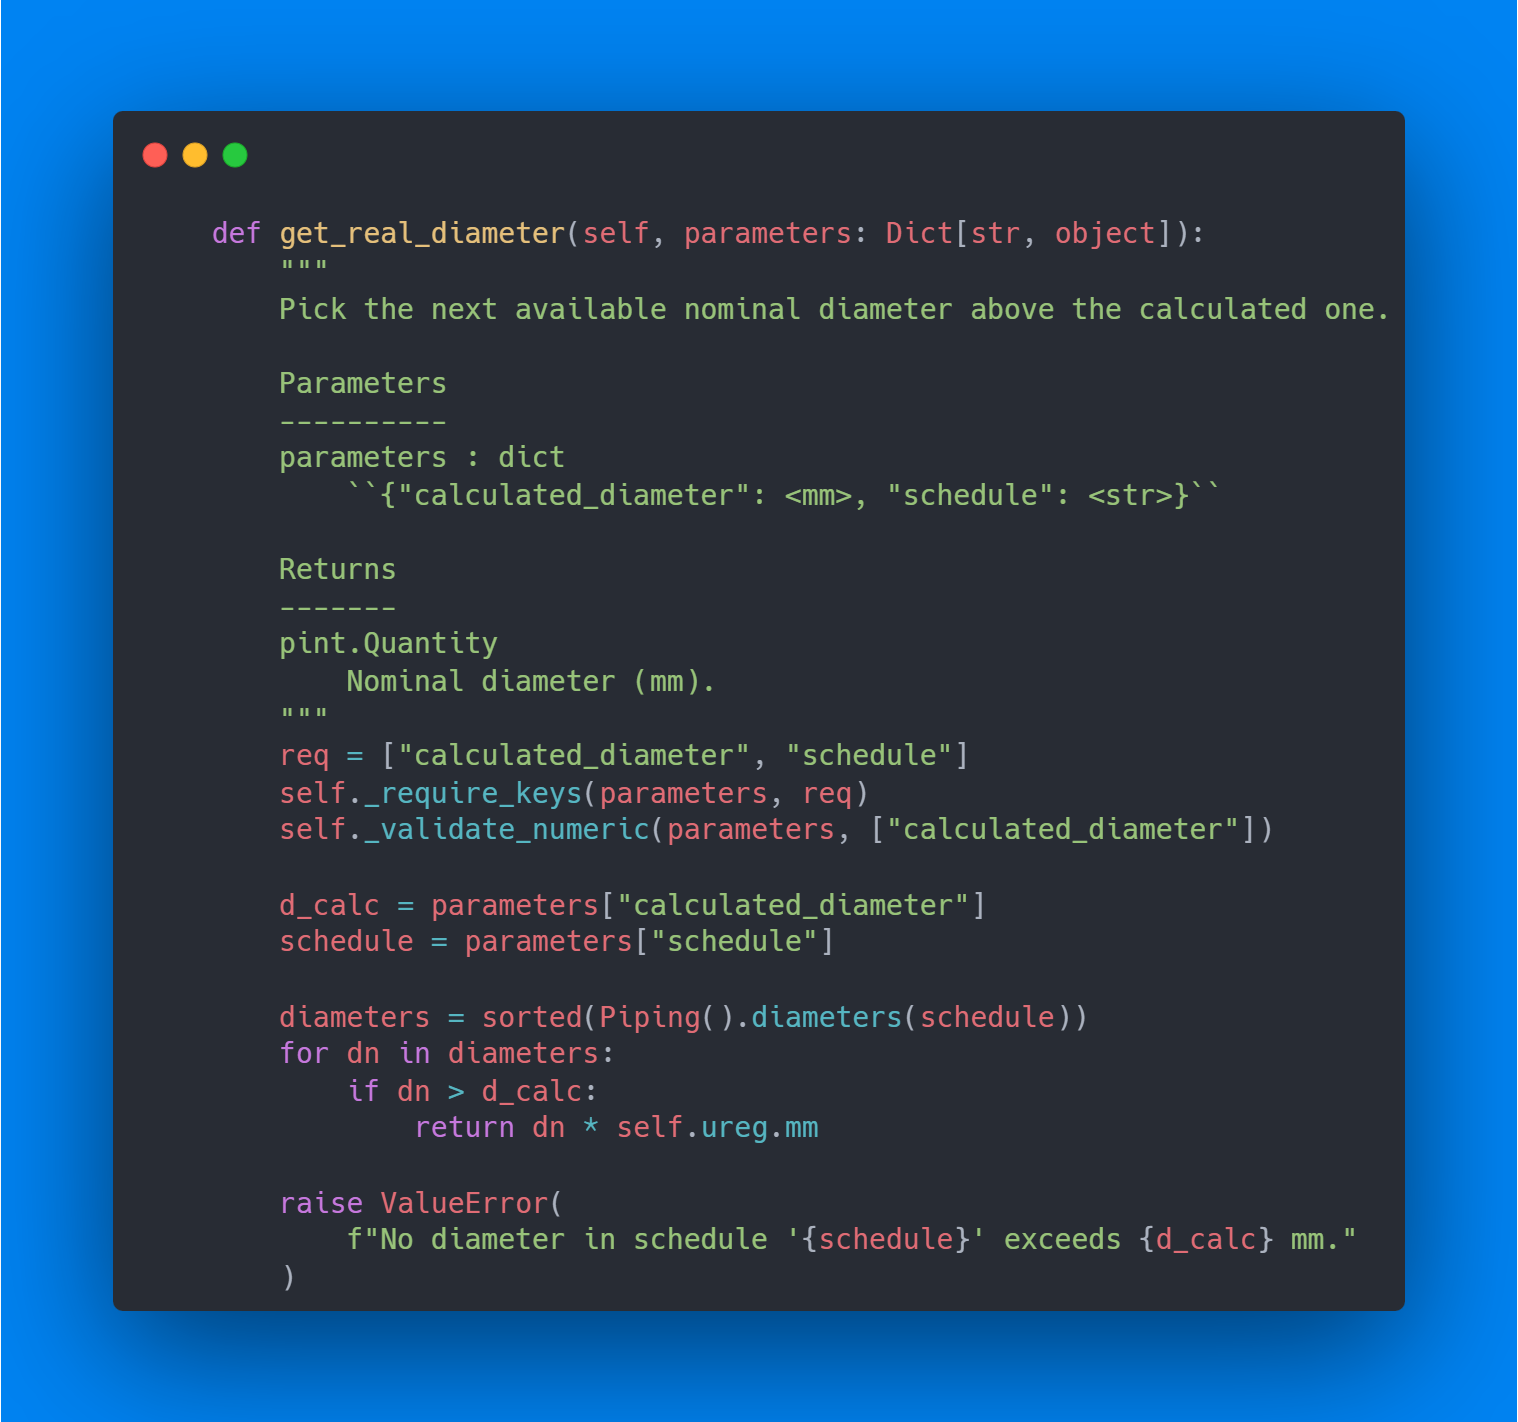
\includegraphics[width=\linewidth]{media/cap4_funcao_get_real_diameter.png}
    \fonte{Elaboração própria (2026).}
\end{figure}

\subsection{Reatores}

Reatores são equipamentos projetados para promover reações químicas, convertendo reagentes em produtos sob condições controladas de operação.

Modelos ideais como \textit{CSTR}, \textit{PFR} e batelada fornecem limites úteis para projeto e análise de desempenho. As variáveis centrais envolvidas no projeto de reatores incluem conversão dos reagentes, seletividade e rendimento (em caso de múltiplas reações), velocidade de reação, tempo de residência, volume do reator e condições de operação (temperatura, pressão). Industrialmente, o correto dimensionamento de reatores afeta diretamente a capacidade produtiva, a qualidade do produto e a segurança, especialmente no controle de remoção de calor em reações exotérmicas. A cinética química depende fortemente da temperatura (lei de Arrhenius) e da forma funcional da taxa de reação (ordem de reação, efeitos de inibição, presença de inertes, variação volumétrica em fase gasosa etc.). Erros na previsão de conversão ou no cálculo do volume reacional podem levar a baixa seletividade, formação de pontos quentes (\textit{hot spots}) e riscos operacionais. A base teórica conjuga balanços de massa por componente com leis cinéticas apropriadas, integradas no espaço (\textit{PFR}) ou no tempo de residência (\textit{CSTR}), podendo incluir balanço de energia quando o regime térmico é relevante \cite{fogler2009,levenspiel2000}.

No escopo deste projeto, são considerados reatores isotérmicos e monofásicos (todos os reagentes e produtos em uma única fase, líquida ou gasosa). O código rejeita misturas de componentes em estados físicos diferentes, a fim de garantir a validade dos balanços e do coeficiente de variação volumétrica utilizado para o estado atual dos módulos de cálculo para reatores.

A Tabela \ref{tab:unidades-reatores-estequiometria} padroniza a leitura dimensional das Equações \ref{eq:razao_reagente} a \ref{eq:dilution_factor}. Assim, os parágrafos seguintes se concentram no papel físico de cada relação.

\begin{table}[H]
    \centering
    \caption{Unidades e natureza dos símbolos nas relações estequiométricas e cinéticas de reatores}
    \label{tab:unidades-reatores-estequiometria}
    \begin{tabular}{|p{0.30\textwidth}|p{0.60\textwidth}|}
        \hline
        \textbf{Símbolo} & \textbf{Unidade ou natureza} \\ \hline
        $N_{i0}$ & Vazão molar, por exemplo $\mathrm{mol/s}$. \\ \hline
        $\nu_i$, $\nu_A$, $\nu_P$, $\nu_R$ & Coeficientes estequiométricos adimensionais. \\ \hline
        $C_i$, $C_{i0}$, $C_{A0}$ & Concentração molar, por exemplo $\mathrm{mol/m^3}$. \\ \hline
        $X$ & Conversão adimensional. \\ \hline
        $y_{A0}$ & Fração molar adimensional do reagente limitante na alimentação. \\ \hline
        $\varepsilon$ & Coeficiente de variação volumétrica adimensional. \\ \hline
        $\psi$ & Fator de diluição adimensional. \\ \hline
        $P$, $P_0$ & Pressões em unidades coerentes entre si, usadas apenas na razão $P_0/P$. \\ \hline
        $T$, $T_0$ & Temperaturas absolutas em $\mathrm{K}$, usadas apenas na razão $T/T_0$. \\ \hline
        $r$ ou $-r_A$ & Taxa molar de reação por volume de reator, por exemplo $\mathrm{mol/(m^3\,s)}$. \\ \hline
        $k$ & Constante cinética com unidades definidas pela ordem global da reação. \\ \hline
    \end{tabular}
\end{table}

Algumas lógicas gerais se aplicam a todos os tipos de reatores implementados. Por exemplo, a determinação do reagente limitante identifica o reagente cuja disponibilidade inicial por unidade estequiométrica é a menor entre os reagentes presentes. Em termos de cálculo, percorrem-se apenas os reagentes (coeficientes estequiométricos negativos), calculando conforme a Equação \ref{eq:razao_reagente}:
\begin{equation}
\mathrm{razao}_{i} = \frac{N_{i0}}{|\nu_i|}
\label{eq:razao_reagente}
\end{equation}
O quociente compara a disponibilidade molar de cada reagente por unidade estequiométrica. O valor absoluto $|\nu_i|$ evita a inversão de sinal causada pela convenção negativa dos reagentes; o reagente com menor valor de $\mathrm{razao}_{i}$ é o limitante \cite{felder2005}.

\begin{figure}[H]
    \centering
    \caption{Código da função \textit{determine\_limiting\_reagent()} – Parte 1/2}
    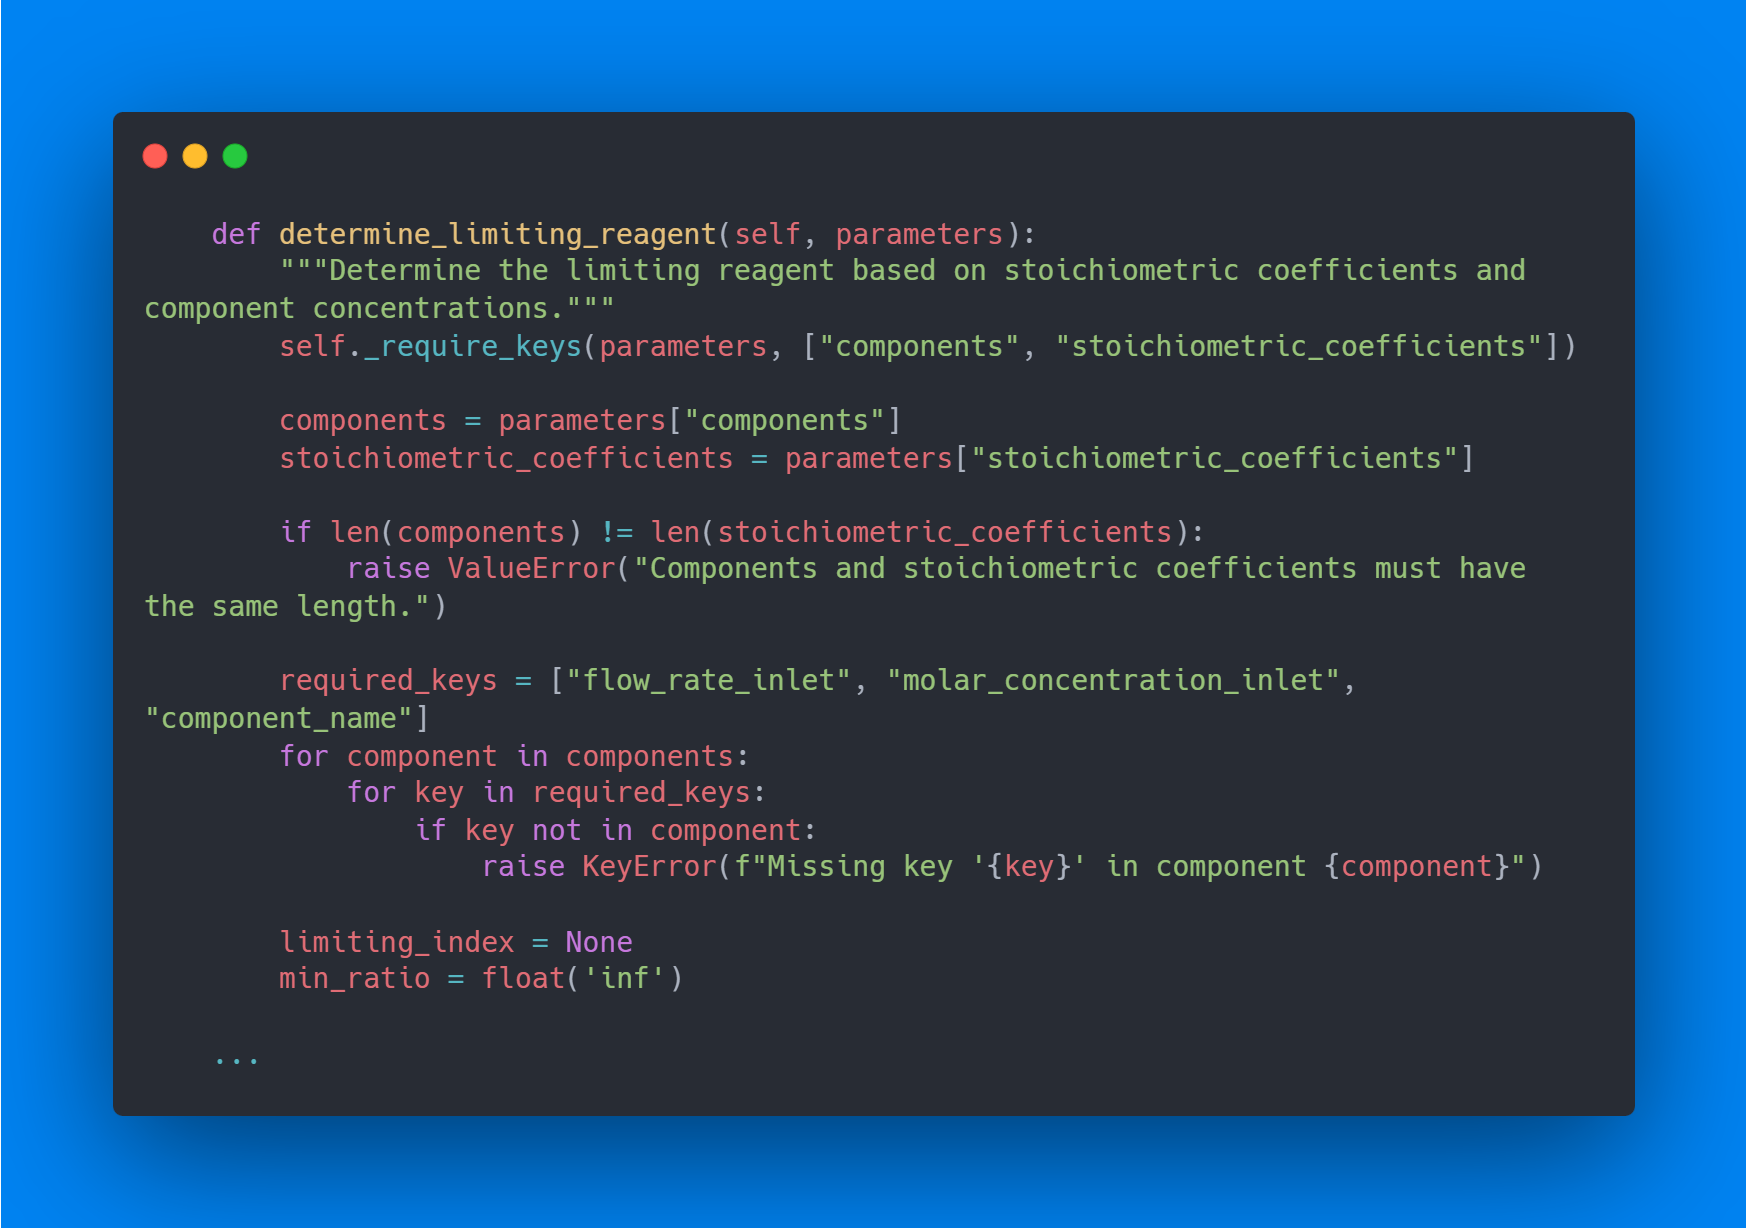
\includegraphics[width=\linewidth]{media/cap4_funcao_determine_limiting_reagent_parte_um.png}
    \fonte{Elaboração própria (2026).}
\end{figure}

\begin{figure}[H]
    \centering
    \caption{Código da função \textit{determine\_limiting\_reagent()} – Parte 2/2}
    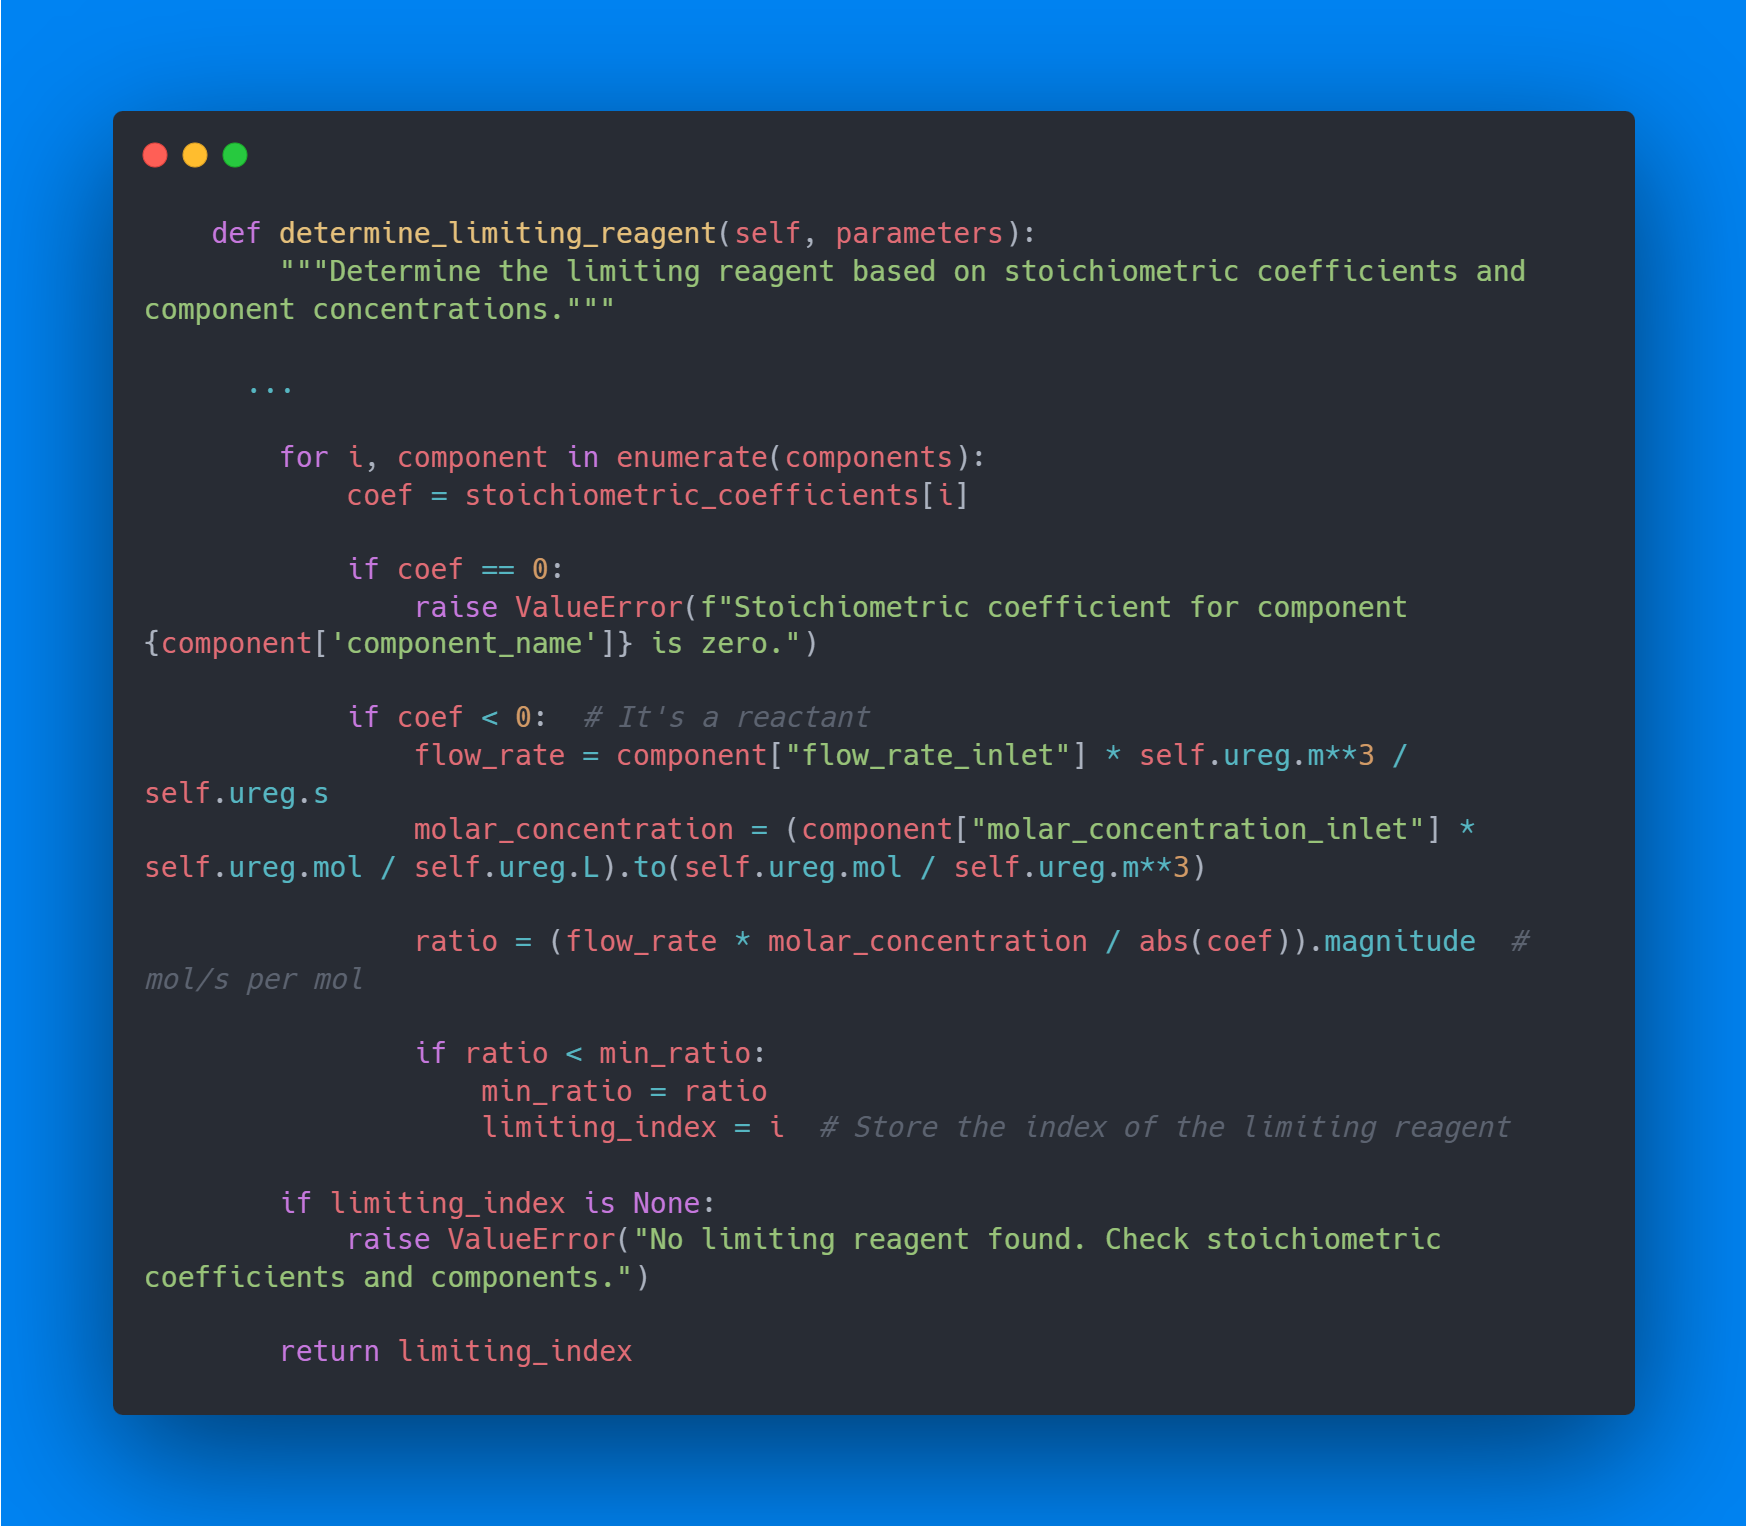
\includegraphics[width=\linewidth]{media/cap4_funcao_determine_limiting_reagent_parte_dois.png}
    \fonte{Elaboração própria (2026).}
\end{figure}

A velocidade de reação é modelada, em geral, por uma lei de potência do tipo:

\begin{equation}
r = k \cdot \prod_{}^{} C_{i}^{n_{i}}
\label{eq:rate_law}
\end{equation}

A Equação \ref{eq:rate_law} representa uma lei de potência: cada concentração entra elevada à sua ordem de velocidade, e $k$ assume a unidade necessária para que o produto resulte em taxa volumétrica de reação.

\begin{figure}[H]
    \centering
    \caption{Código da função \textit{\_calculate\_concentration\_and\_rate()} – Trecho da velocidade da reação}
    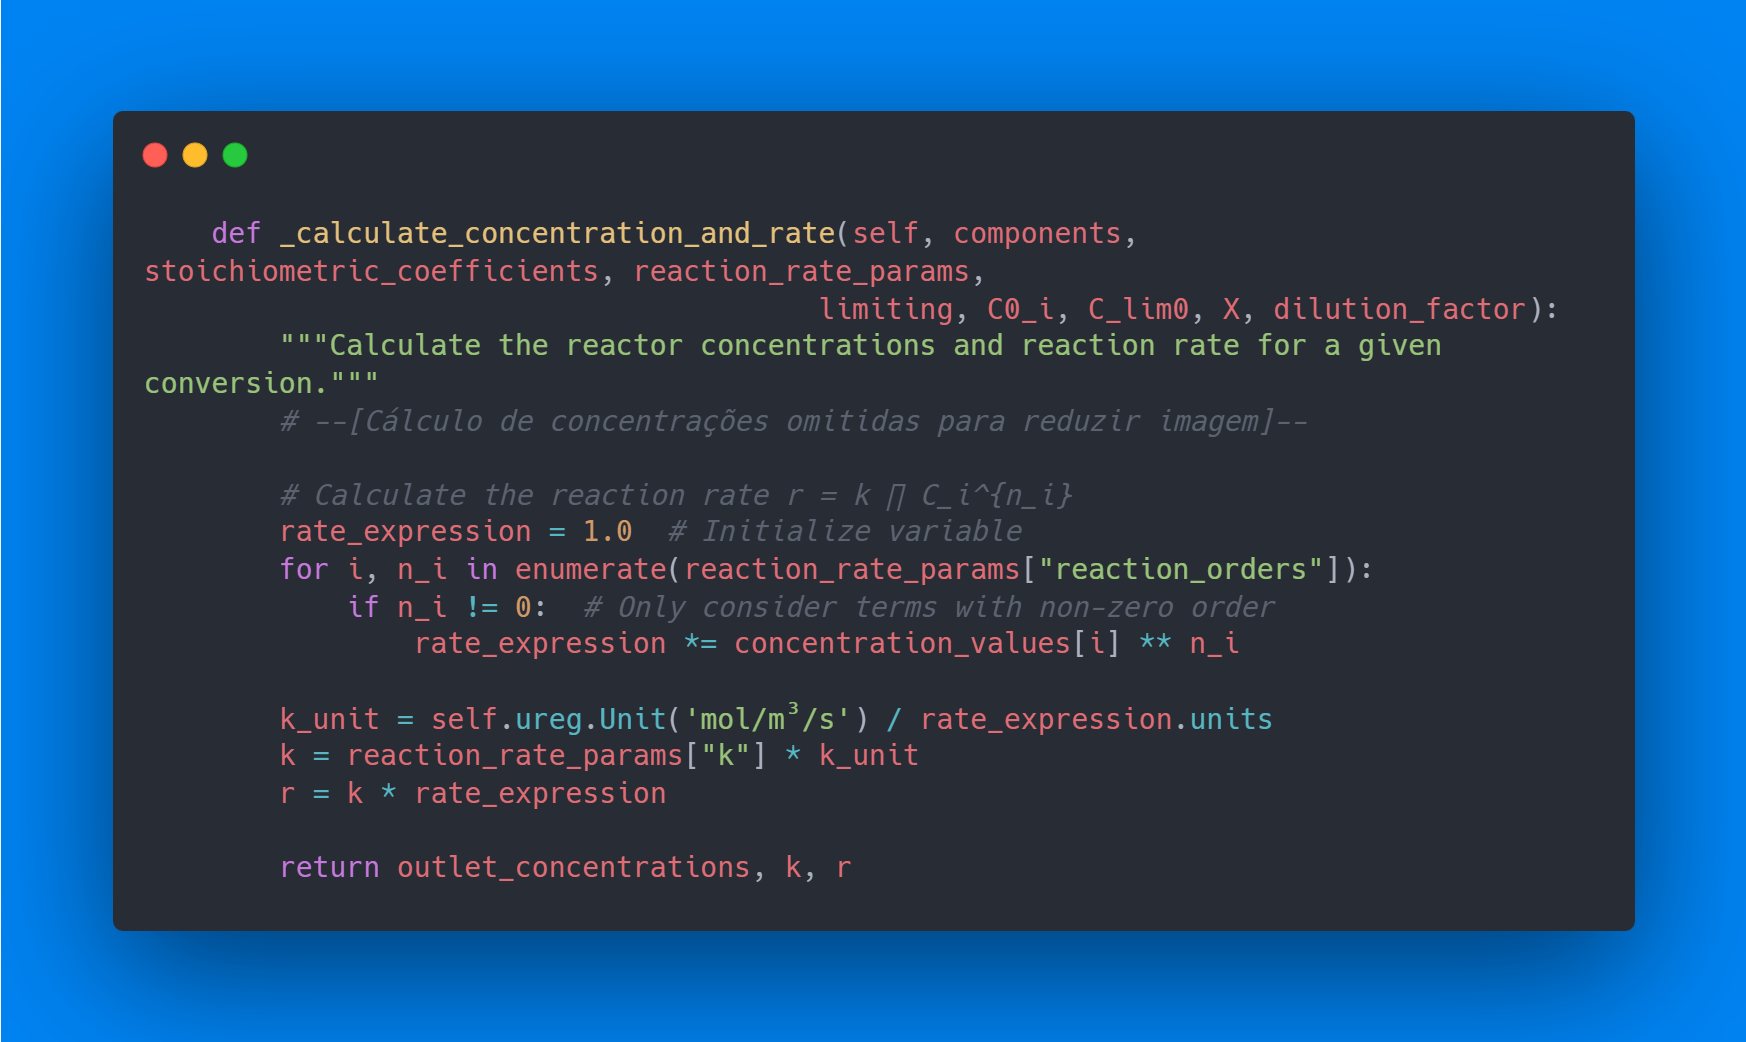
\includegraphics[width=\linewidth]{media/cap4_funcao_calculate_concentration_and_rate_velocidade.png}
    \fonte{Elaboração própria (2026).}
\end{figure}

A integração da cinética com a estequiometria é feita via conversão $X$ do reagente limitante. Os balanços estequiométricos relacionam as concentrações de saída de cada componente à conversão $X$. Para cada componente $i$ na reação, tem-se a seguinte relação geral: o termo estequiométrico é positivo para formação (produtos), negativo para consumo (reagentes) e nulo para inertes.

\begin{equation}
C_{i} = \frac{C_{i0} + \left( \frac{\nu_i}{|\nu_A|} \cdot C_{A0} \cdot X \right)}{\psi}
\label{eq:conc_stoich}
\end{equation}

A Equação \ref{eq:conc_stoich} ajusta a concentração de cada componente pela conversão do reagente limitante. O numerador representa consumo ou formação estequiométrica, enquanto o denominador aplica a diluição total do meio.

\begin{figure}[H]
    \centering
    \caption{Código da função \textit{\_calculate\_concentration\_and\_rate()} – Trecho da concentração dos componentes}
    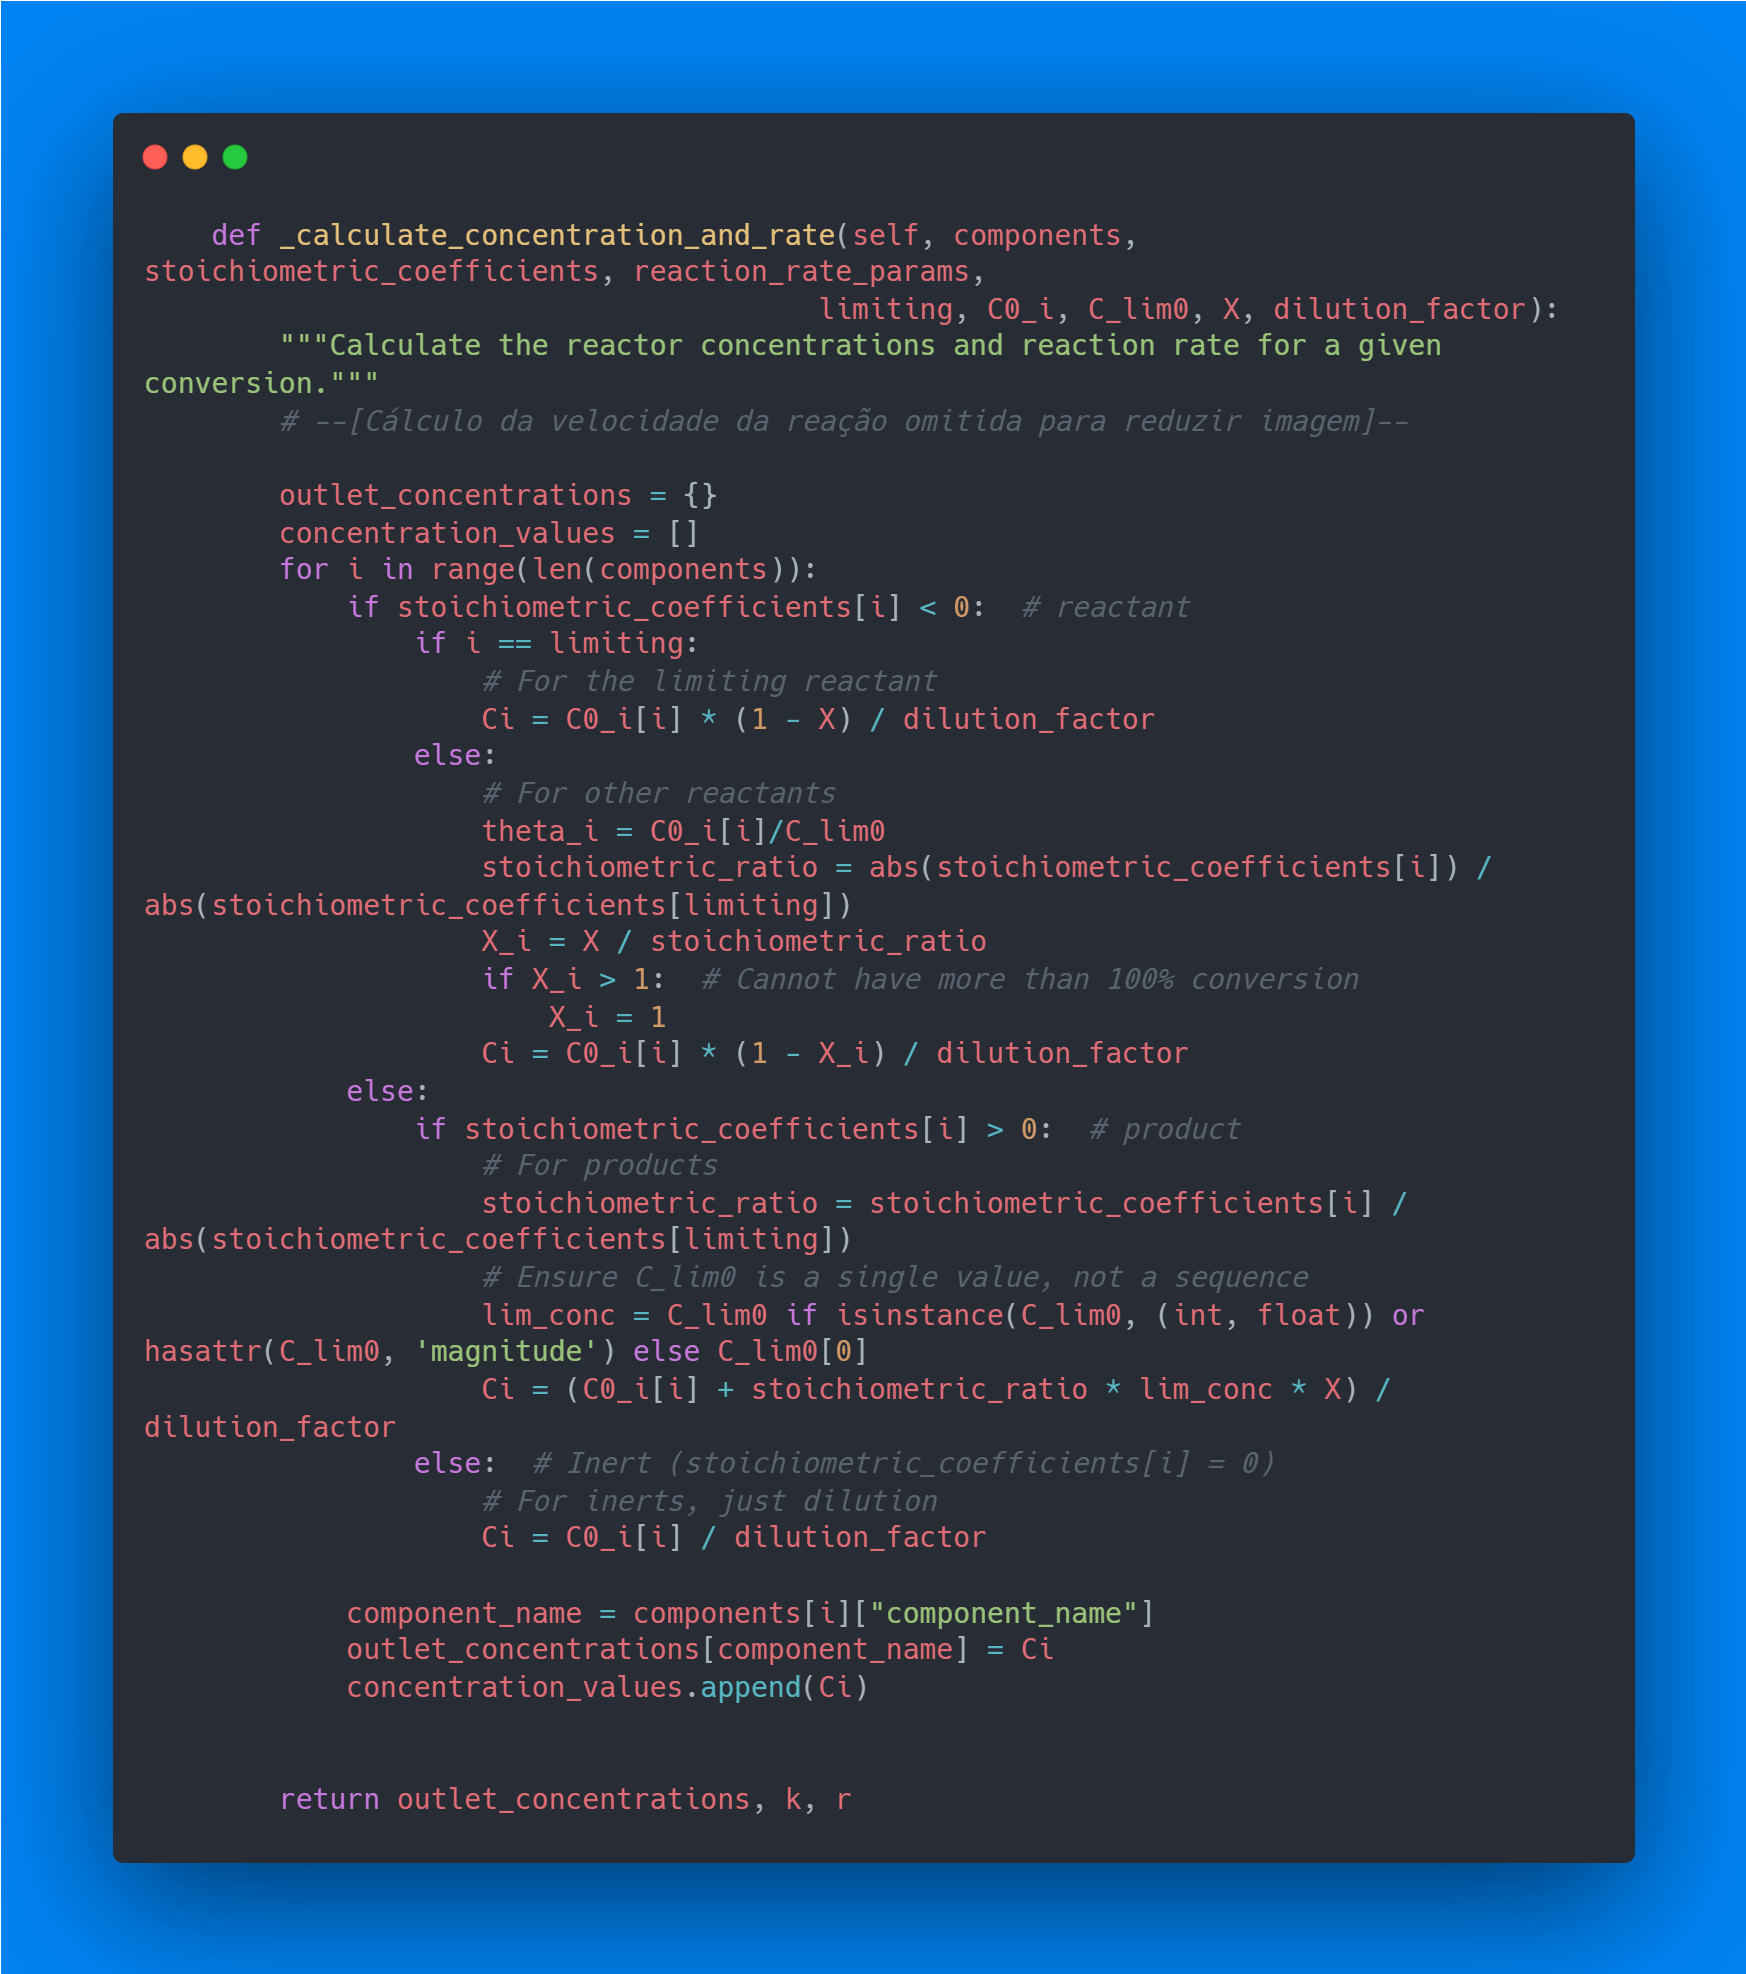
\includegraphics[width=\linewidth]{media/cap4_funcao_calculate_concentration_and_rate_componentes.png}
    \fonte{Elaboração própria (2026).}
\end{figure}

Para determinação do coeficiente de variação volumétrica para reações gasosas, a Equação \ref{eq:epsilon_def} deve ser utilizada.

\begin{equation}
\varepsilon = y_{A0} \cdot \frac{\sum_{\nu_i>0} \nu_i - \sum_{\nu_i<0} |\nu_i|}{|\nu_{A}|}
\label{eq:epsilon_def}
\end{equation}

O numerador compara a quantidade estequiométrica formada e consumida na fase gasosa, normalizada pelo reagente limitante. O sinal de $\varepsilon$ indica expansão ou contração molar associada à reação.

\begin{equation}
\psi = ( 1 + \varepsilon X ) \frac{P_{0}}{P} \frac{T}{T_{0}}
\label{eq:dilution_factor}
\end{equation}

\begin{figure}[H]
    \centering
    \caption{Código da função \textit{\_calculate\_dilution\_factor()}}
    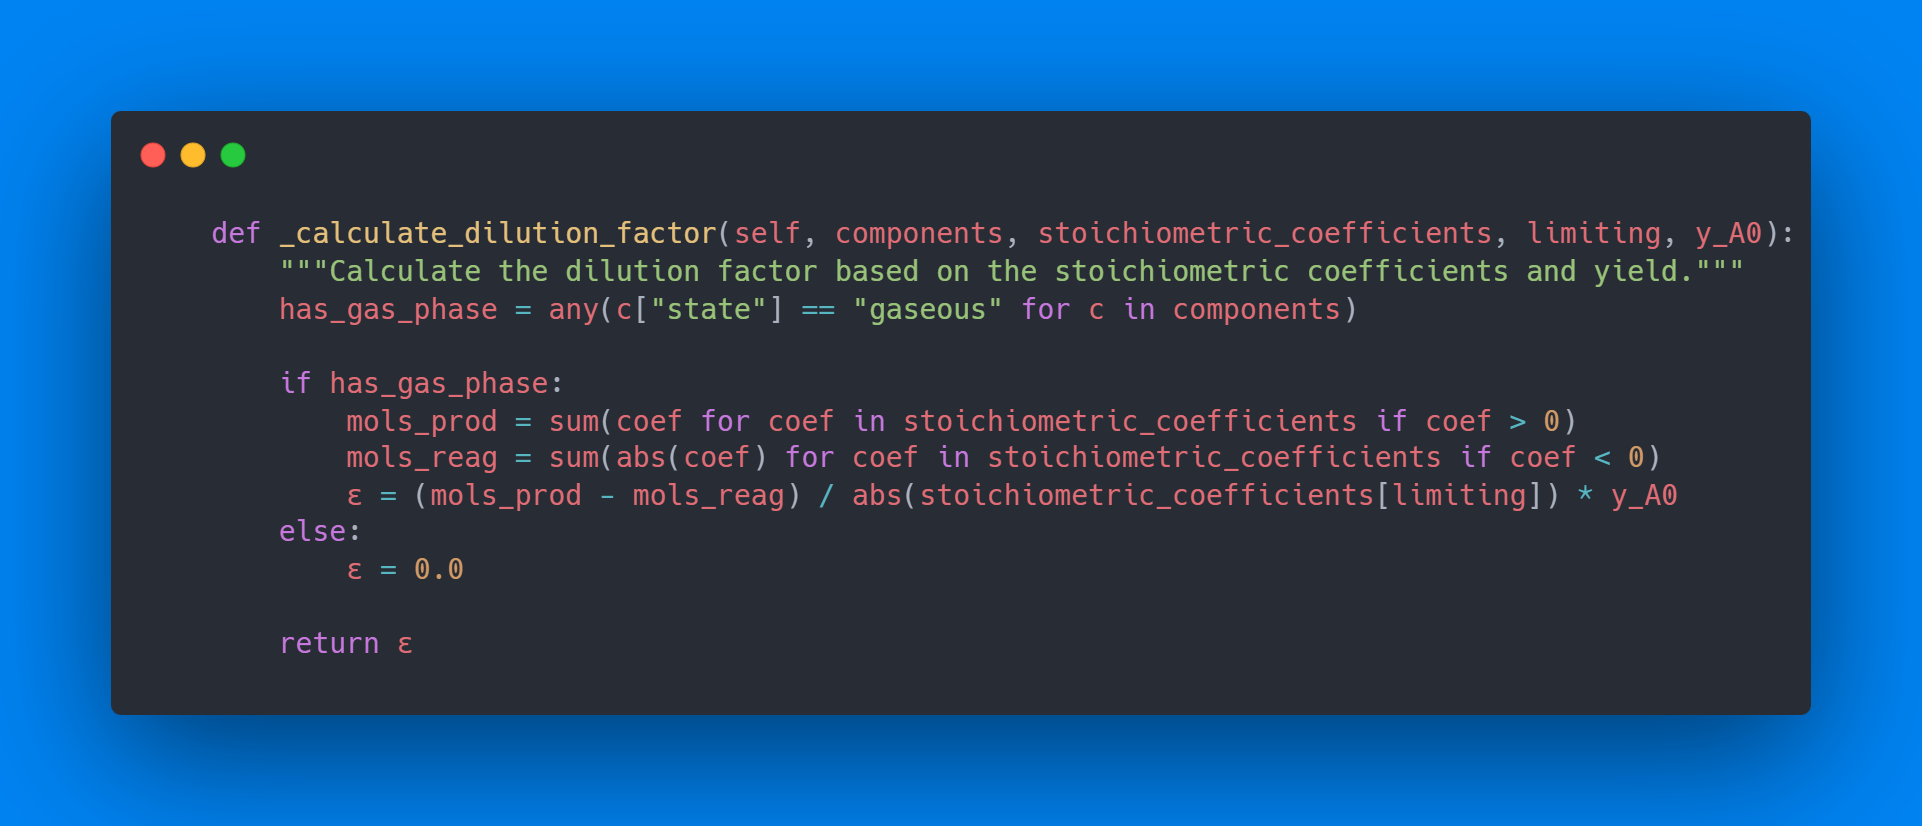
\includegraphics[width=\linewidth]{media/cap4_funcao_calculate_dilution_factor.png}
    \fonte{Elaboração própria (2026).}
\end{figure}

Onde $\varepsilon$ representa a variação volumétrica ou molar por mol de $A$ reagido, podendo indicar expansão ou contração conforme a estequiometria e a fase gasosa. O fator $\psi$ agrega a variação volumétrica estequiométrica (via $\varepsilon X$) e as correções de pressão e temperatura em relação às condições iniciais \cite{levenspiel2000}. Essas relações estequiométricas permitem calcular as concentrações de saída de todos os componentes a partir da conversão $X$ do reagente limitante, sendo a base para os balanços nos diferentes modelos de reatores.

\subsubsection{Reator do Tipo \textit{CSTR}}

O reator do tipo \textit{CSTR} é um tanque agitado operando em regime contínuo. Assume-se mistura completa no interior do tanque (composição uniforme em todo o volume). A conversão é desenvolvida integralmente dentro do volume do reator, dependendo do balanço entre a cinética de reação e o tempo de residência dos reagentes no tanque.

No sistema implementado, são suportados três casos de uso: (i) conversão desejada e cinética conhecidas (calcula-se o volume do reator necessário), (ii) volume disponível e cinética conhecidas (calcula-se a conversão atingida) e (iii) tempo de residência e cinética conhecidos (calcula-se a conversão atingida). As saídas calculadas pelo algoritmo incluem, entre outros: conversão do reagente limitante $X$, vazão molar do reagente limitante na entrada $F_{A0}$, vazão volumétrica total na saída $Q_{T}$, volume do reator $V$, taxa de reação $r$ no interior, concentrações de saída $C_{i,\mathrm{saida}}$, fator de diluição $\psi$, coeficiente de variação volumétrica $\varepsilon$ e tempo de residência $\tau$.

A Tabela \ref{tab:unidades-cstr} resume as unidades locais da sequência de cálculo do \textit{CSTR}; essas definições valem para as Equações \ref{eq:molar_flow_in} a \ref{eq:volume_calc}.

\begin{table}[H]
    \centering
    \caption{Unidades e natureza dos símbolos na sequência de cálculo do \textit{CSTR}}
    \label{tab:unidades-cstr}
    \begin{tabular}{|p{0.30\textwidth}|p{0.60\textwidth}|}
        \hline
        \textbf{Símbolo} & \textbf{Unidade ou natureza} \\ \hline
        $N_{i0}$, $F_{A0}$ & Vazão molar, por exemplo $\mathrm{mol/s}$. \\ \hline
        $Q_i$, $Q_T$ & Vazão volumétrica, por exemplo $\mathrm{m^3/s}$. \\ \hline
        $C_{i0}$, $C_{i0e}$ & Concentração molar, por exemplo $\mathrm{mol/m^3}$. \\ \hline
        $V$ & Volume do reator, por exemplo $\mathrm{m^3}$. \\ \hline
        $X$ & Conversão adimensional. \\ \hline
        $-r_A$ & Taxa molar de reação por volume de reator, por exemplo $\mathrm{mol/(m^3\,s)}$. \\ \hline
        $\tau$ & Tempo de residência, por exemplo $\mathrm{s}$. \\ \hline
        $f(X)$ em \ref{eq:cstr_obj_function} & Resíduo objetivo: diferença numérica entre conversões adimensionais. \\ \hline
    \end{tabular}
\end{table}

\paragraph{Conversão e Cinética (Cálculo do Volume)}

Passos principais do cálculo:
\begin{itemize}
    \item Identificação do reagente limitante (conforme descrito anteriormente);
    \item Cálculo das vazões molares de entrada pela Equação \ref{eq:molar_flow_in}:
    \begin{equation}
    N_{i 0} = Q_{i} \cdot C_{i 0 e}
    \label{eq:molar_flow_in}
    \end{equation}
    para cada componente, bem como da vazão volumétrica total pela Equação \ref{eq:total_flow}:
    \begin{equation}
    Q_{T} = \sum_{}^{} Q_{i}
    \label{eq:total_flow}
    \end{equation}
    As concentrações iniciais (após mistura das correntes de alimentação) são dadas pela Equação \ref{eq:initial_conc}:
    \begin{equation}
    C_{i 0} = \frac{N_{i 0}}{Q_{T}}
    \label{eq:initial_conc}
    \end{equation}
    \item Cálculo do fator de diluição total $\psi$ com a conversão alvo $X$ (Equação \ref{eq:dilution_factor});
    \item Cálculo da taxa de reação $r$ a partir da constante cinética $k$ e das concentrações na saída (considerando $X$), supondo regime isotérmico \cite{fogler2009};
    \item Aplicação do balanço no \textit{CSTR} para o reagente limitante.
\end{itemize}

Para conversão $X$ conhecida, a equação de \textit{design} é dada por:

\begin{equation}
V = \frac{F_{A 0} \cdot X}{- r_{A}}
\label{eq:cstr_design}
\end{equation}

Nessa expressão, o produto $F_{A0}X$ representa a vazão molar convertida do reagente limitante, e a divisão pela taxa de consumo volumétrica fornece o volume requerido do tanque.

Cálculo do tempo de residência:

\begin{equation}
\tau = \frac{V}{Q_{T}}
\label{eq:residence_time}
\end{equation}

\begin{figure}[H]
    \centering
    \caption{Código da função \textit{\_conversion\_and\_kinetics\_in\_cstr()} – Parte 1/2}
    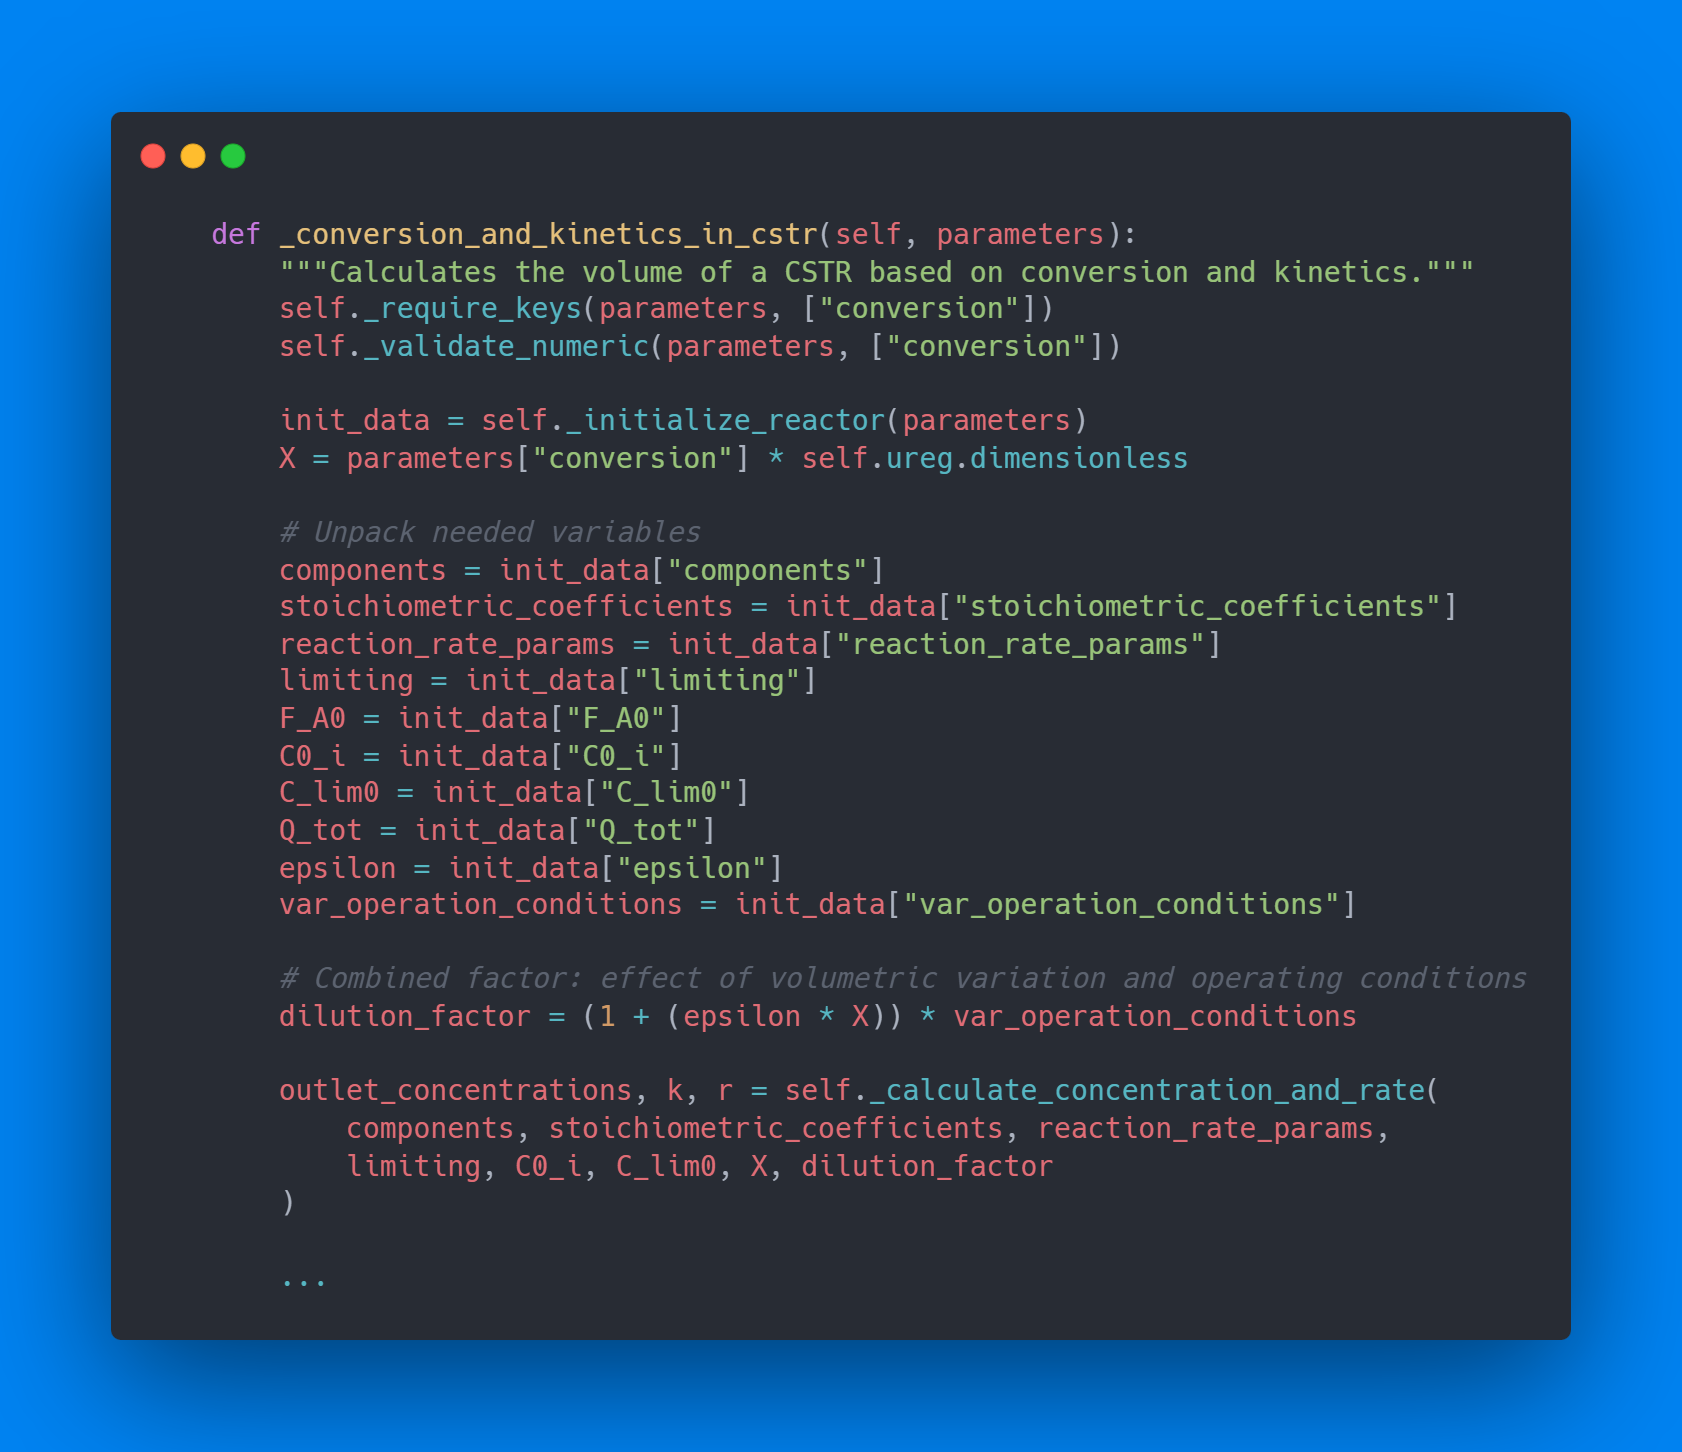
\includegraphics[width=\linewidth]{media/cap4_funcao_conversion_and_kinetics_in_cstr_parte_um.png}
    \fonte{Elaboração própria (2026).}
\end{figure}

\begin{figure}[H]
    \centering
    \caption{Código da função \textit{\_conversion\_and\_kinetics\_in\_cstr()} – Parte 2/2}
    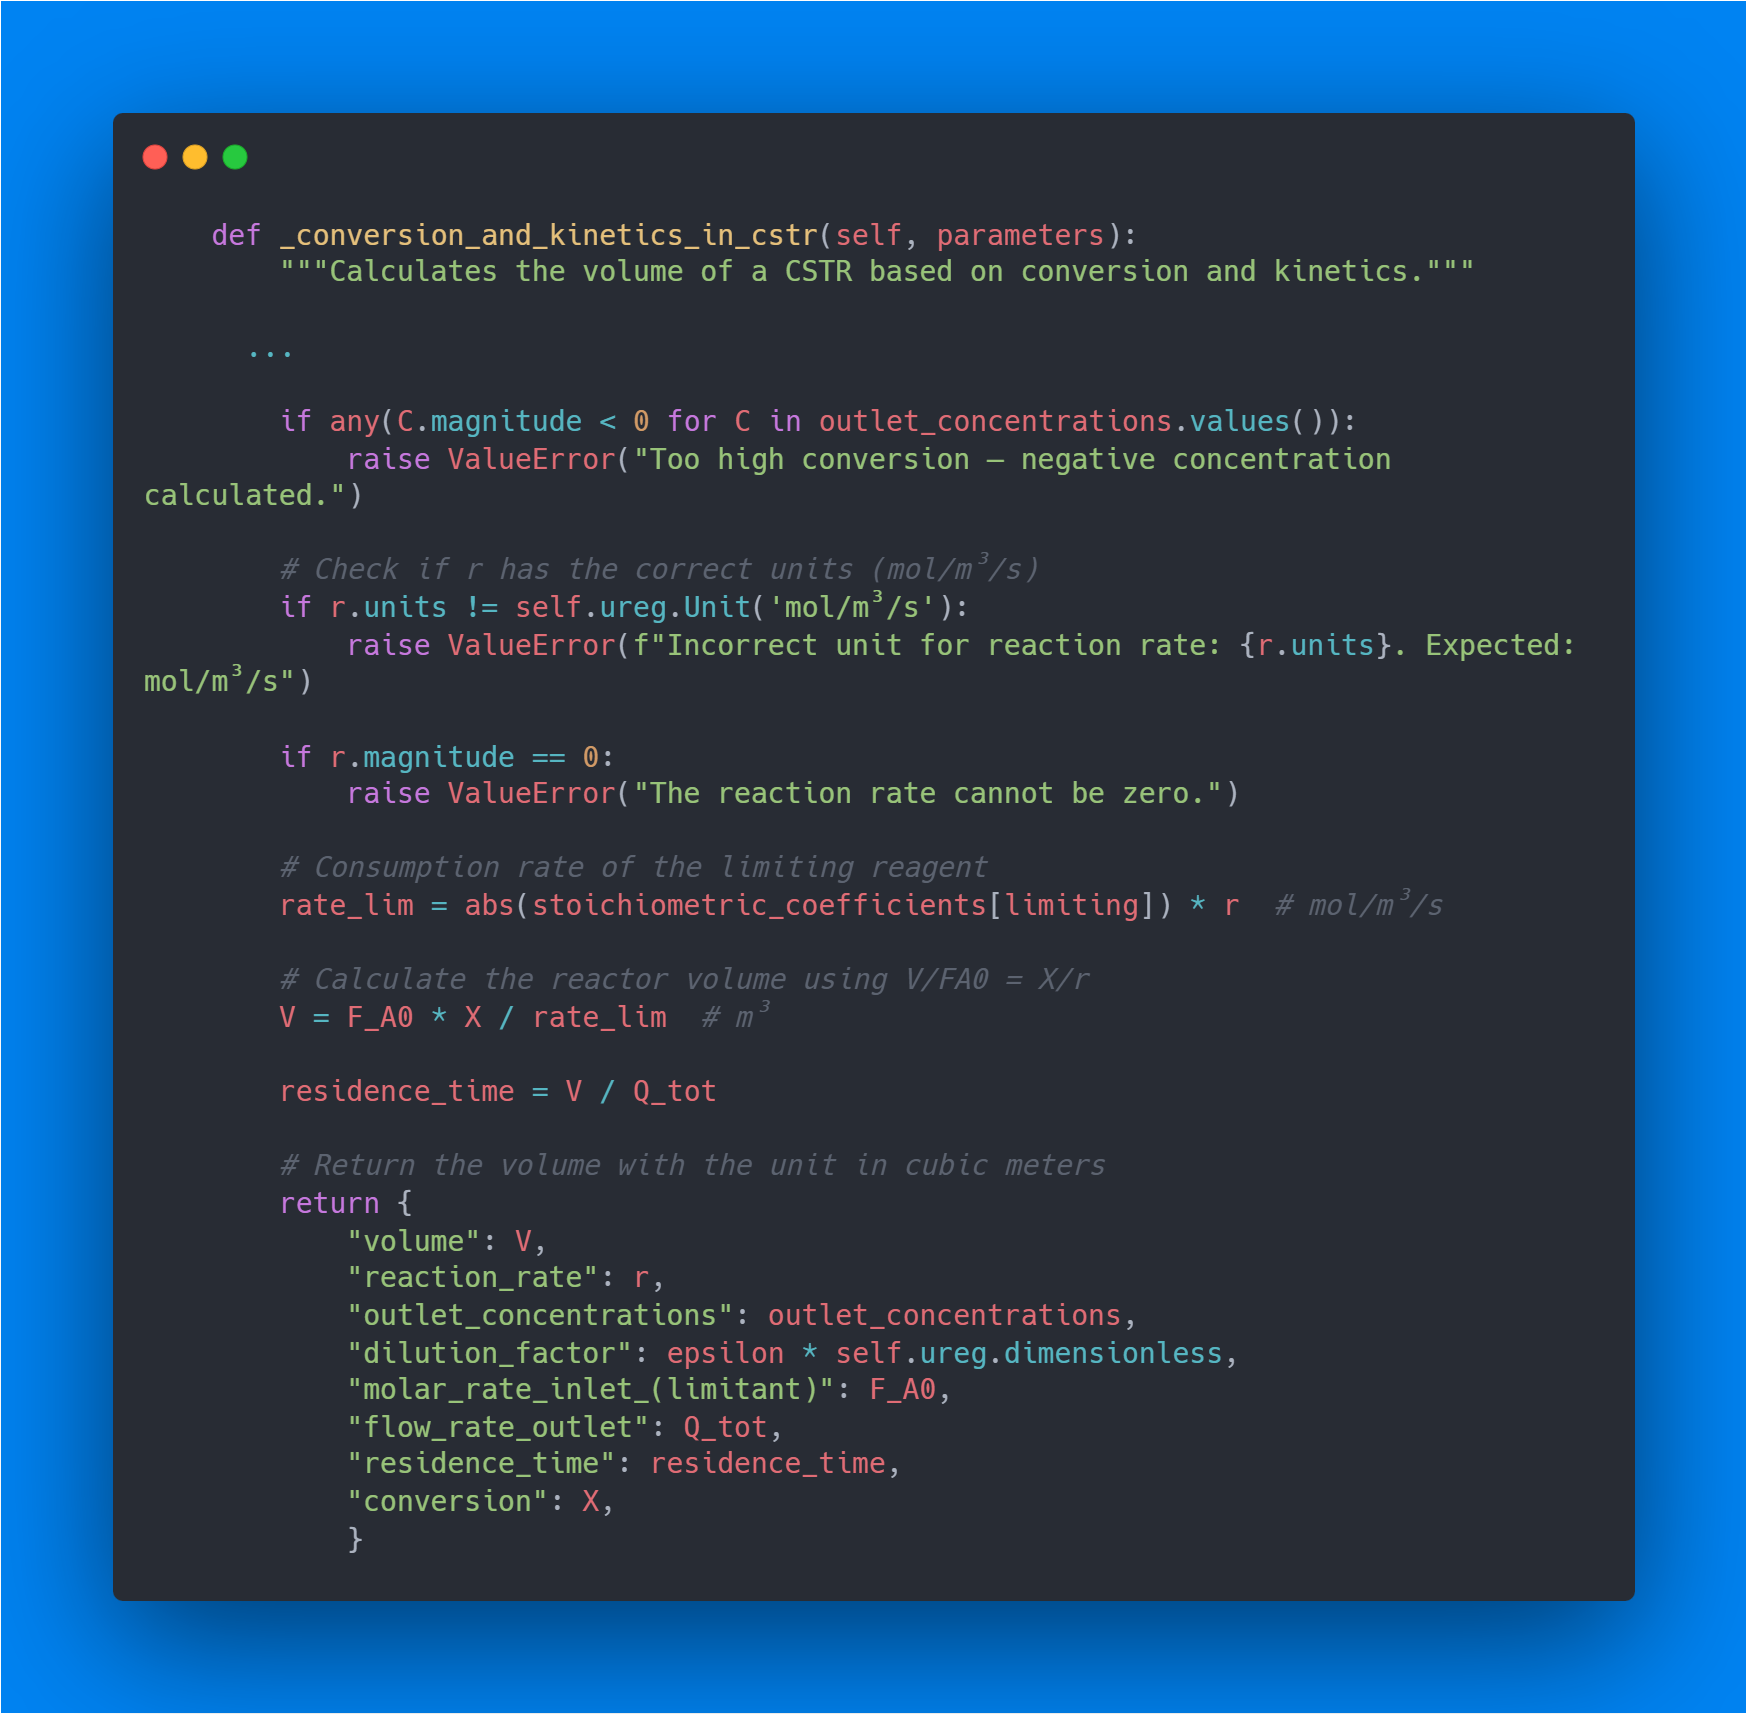
\includegraphics[width=\linewidth]{media/cap4_funcao_conversion_and_kinetics_in_cstr_parte_dois.png}
    \fonte{Elaboração própria (2026).}
\end{figure}

A fim de simplificar as rotinas, utiliza-se a função \textit{\_initialize\_reactor()}, que calcula as concentrações e vazões de cada componente na entrada, bem como o coeficiente de variação volumétrica ou molar, o fator de diluição, as temperaturas e pressões iniciais e finais e o reagente limitante.

\begin{figure}[H]
    \centering
    \caption{Código da função \textit{\_initialize\_reactor()} – Parte 1/2}
    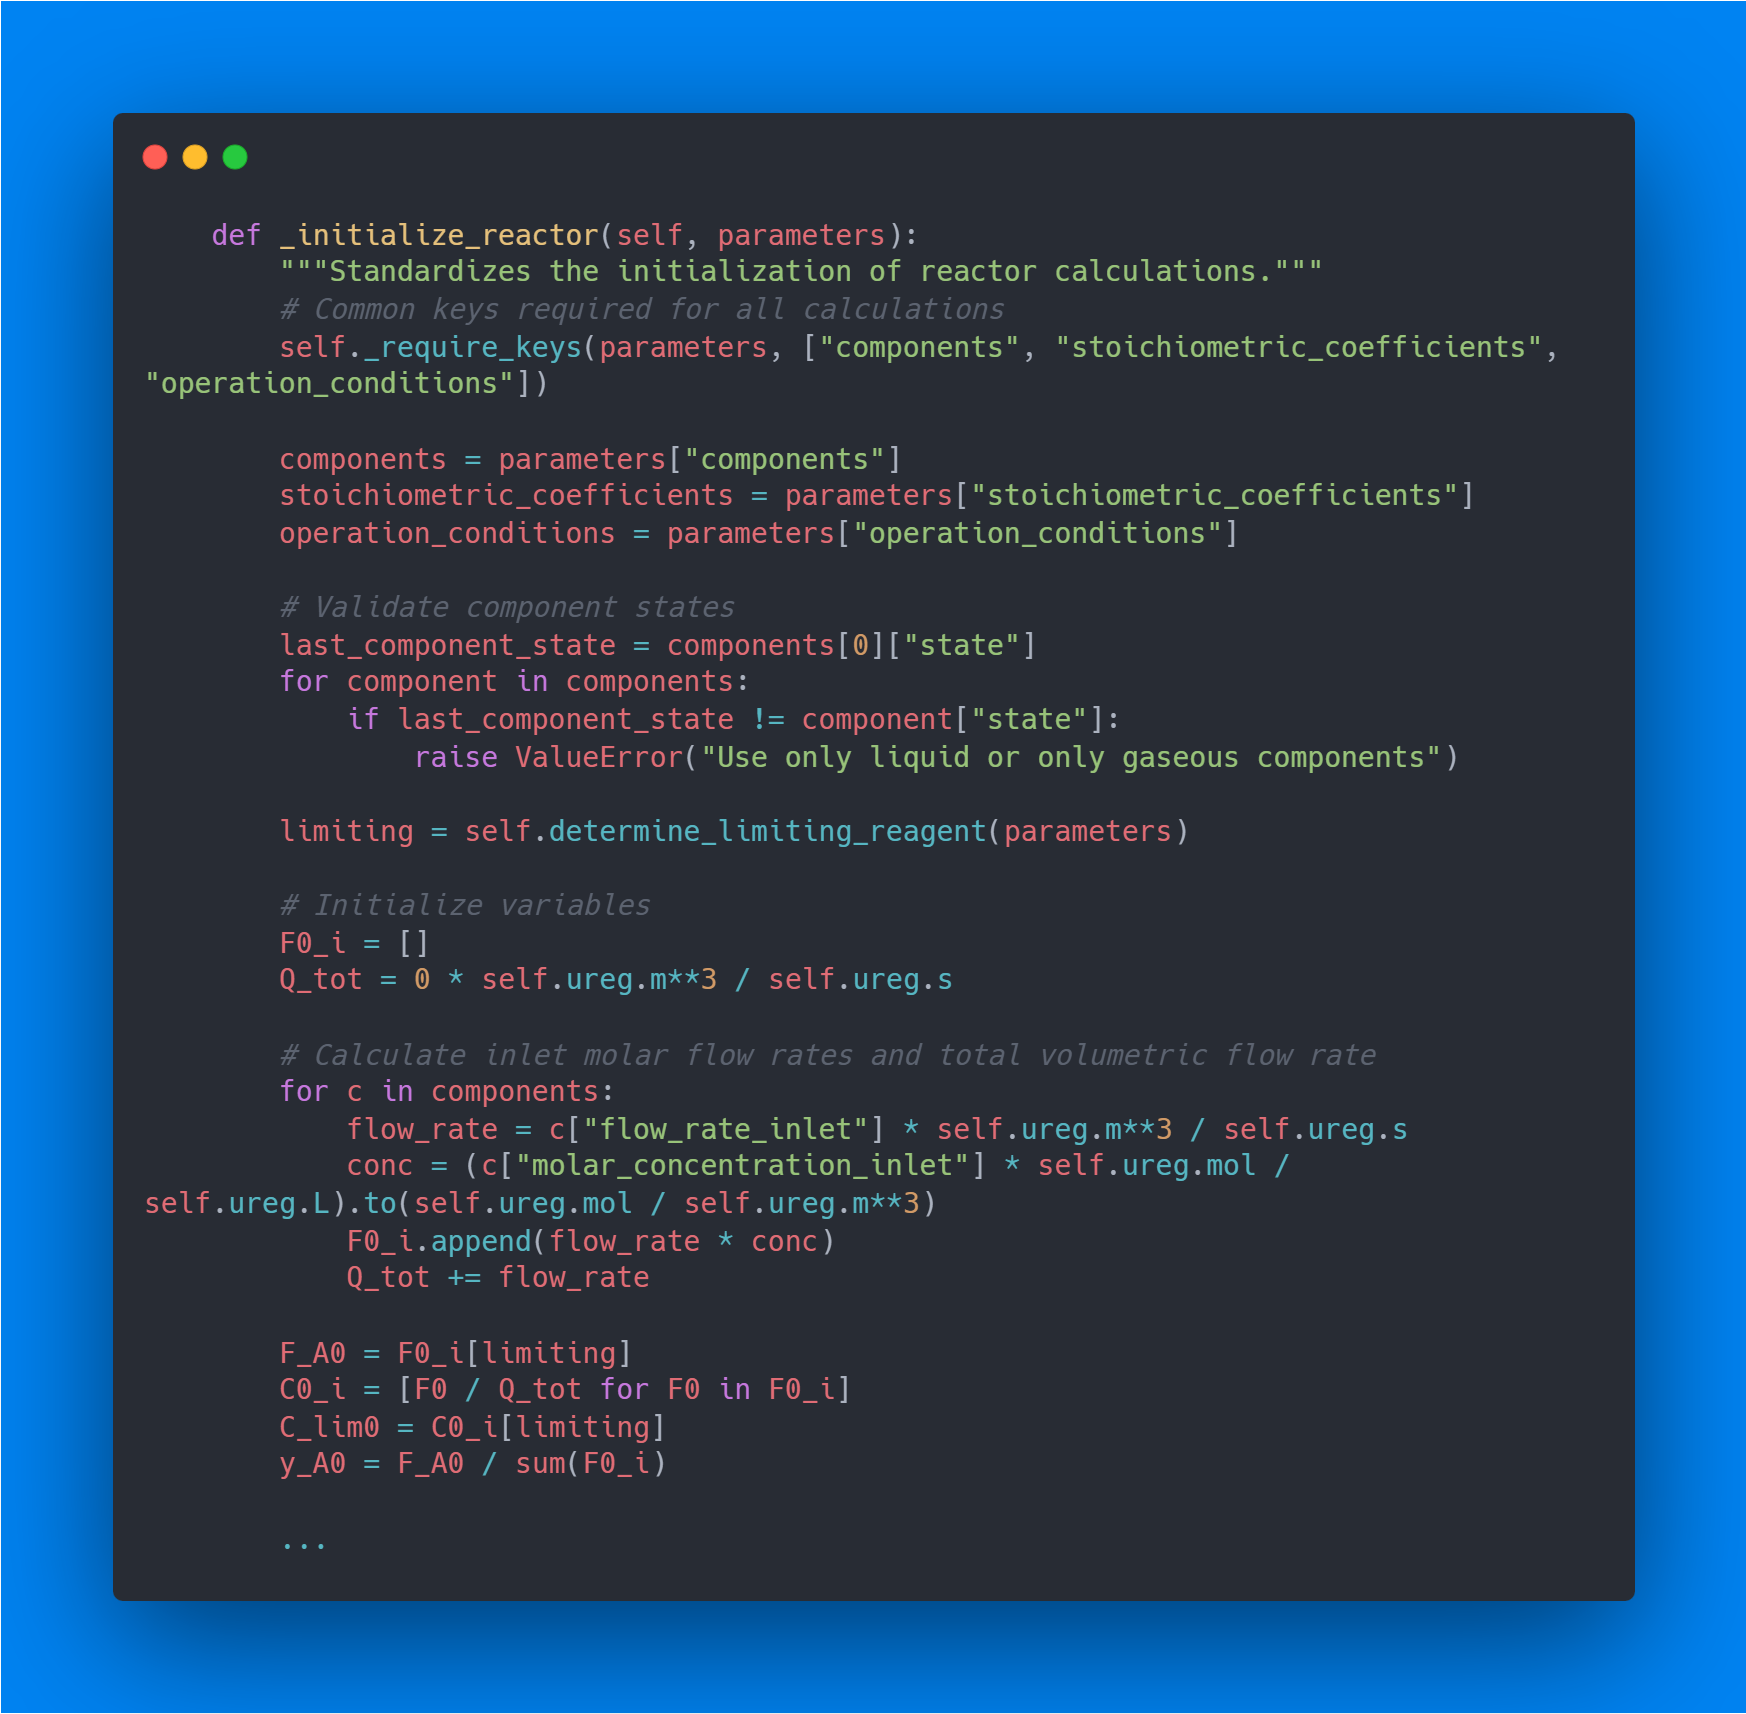
\includegraphics[width=\linewidth]{media/cap4_funcao_initialize_reactor_parte_um.png}
    \fonte{Elaboração própria (2026).}
\end{figure}

\begin{figure}[H]
    \centering
    \caption{Código da função \textit{\_initialize\_reactor()} – Parte 2/2}
    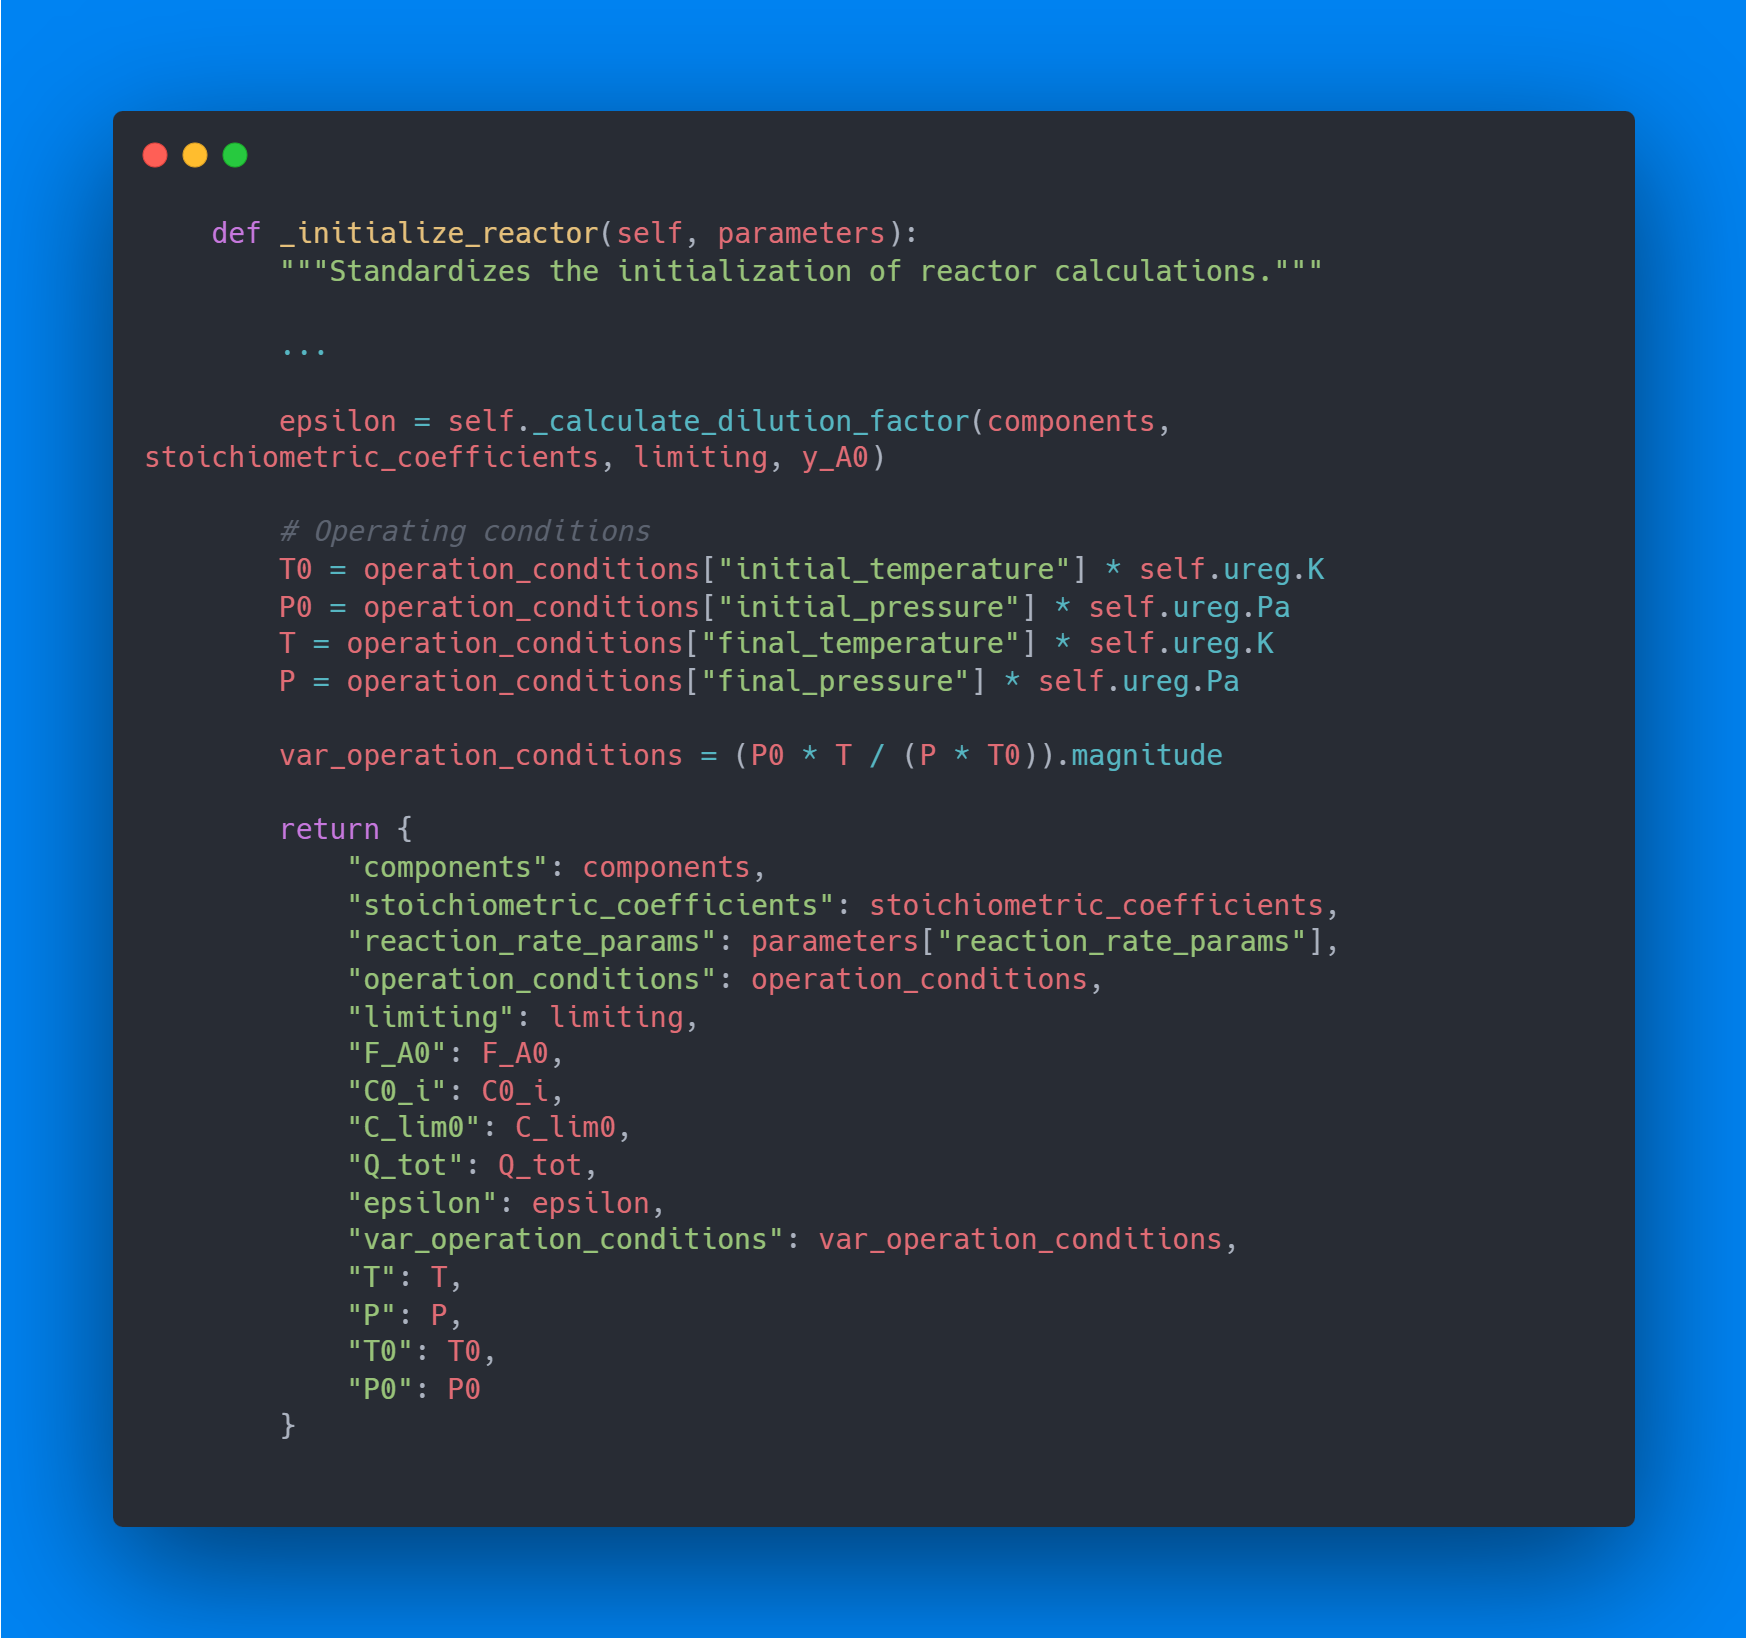
\includegraphics[width=\linewidth]{media/cap4_funcao_initialize_reactor_parte_dois.png}
    \fonte{Elaboração própria (2026).}
\end{figure}

\paragraph{Volume e Cinética (Cálculo da Conversão)}

Nesse caso, são conhecidos o volume do reator $V$ e a cinética (expressão da taxa $r ( C_{i} )$, incluindo $k$). Deseja-se determinar a conversão $X$ atingida no \textit{CSTR}. Isolando $X$ na equação de \textit{design} do \textit{CSTR} obtém-se uma equação implícita. Define-se então uma função objetivo:

\begin{equation}
f ( x ) = \frac{{| v}_{A} | \cdot r_{A} \cdot V}{F_{A 0}} - X
\label{eq:cstr_obj_function}
\end{equation}

Então encontra-se sua raiz na faixa 0<X<1, tipicamente utilizando o método de Brent, dada a monotonicidade esperada de $f ( x )$. A raiz X que satisfaz $f ( x ) = 0$ corresponde à conversão no reator.

\begin{figure}[H]
    \centering
    \caption{Código da função \textit{\_volume\_and\_kinetics\_in\_cstr()} – Parte 1/2}
    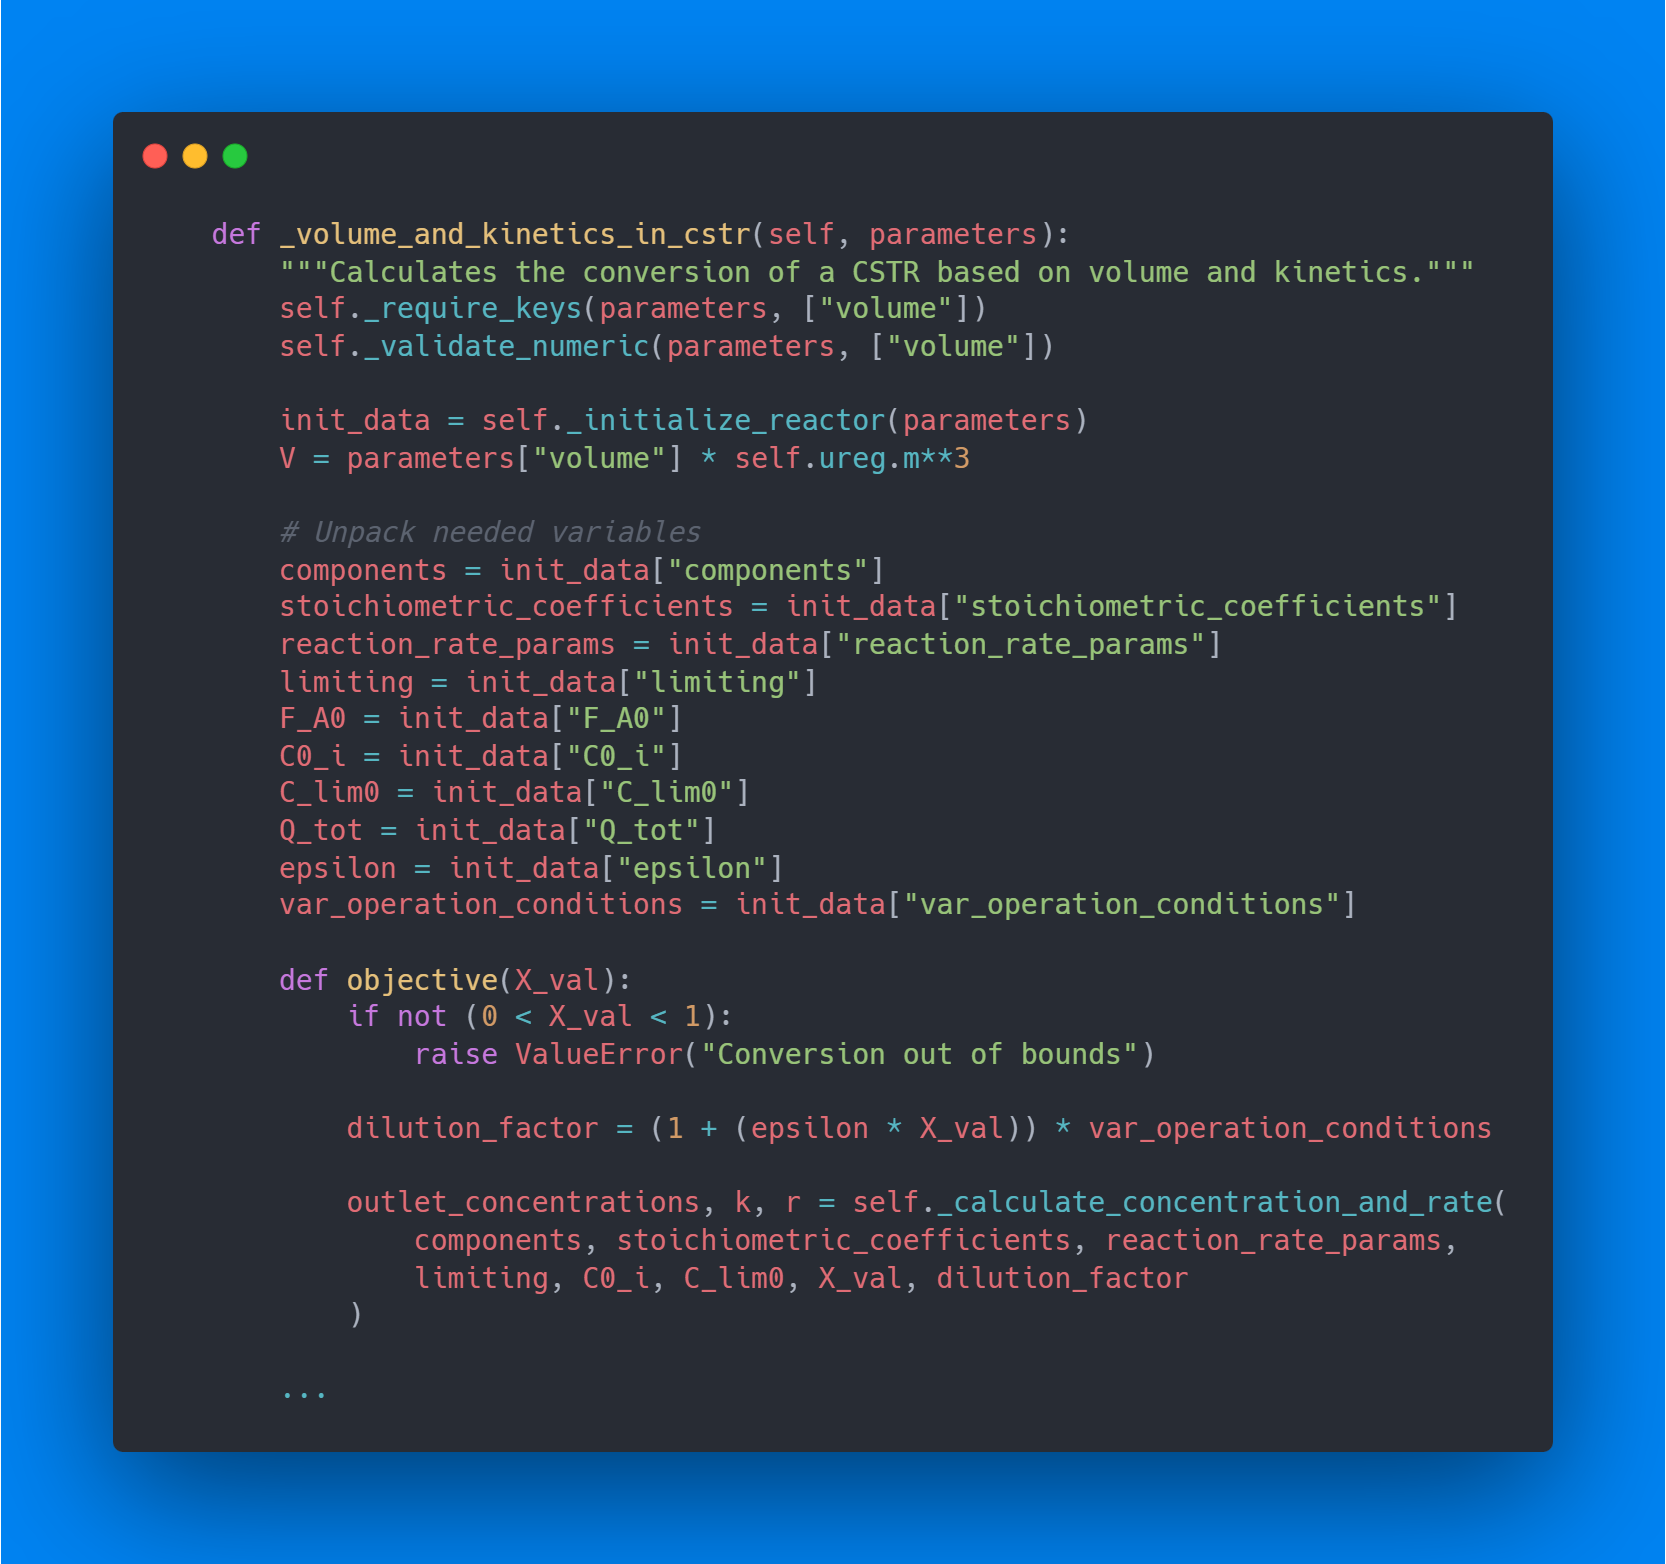
\includegraphics[width=\linewidth]{media/cap4_funcao_volume_and_kinetics_in_cstr_parte_um.png}
    \fonte{Elaboração própria (2026).}
\end{figure}

\begin{figure}[H]
    \centering
    \caption{Código da função \textit{\_volume\_and\_kinetics\_in\_cstr()} – Parte 2/2}
    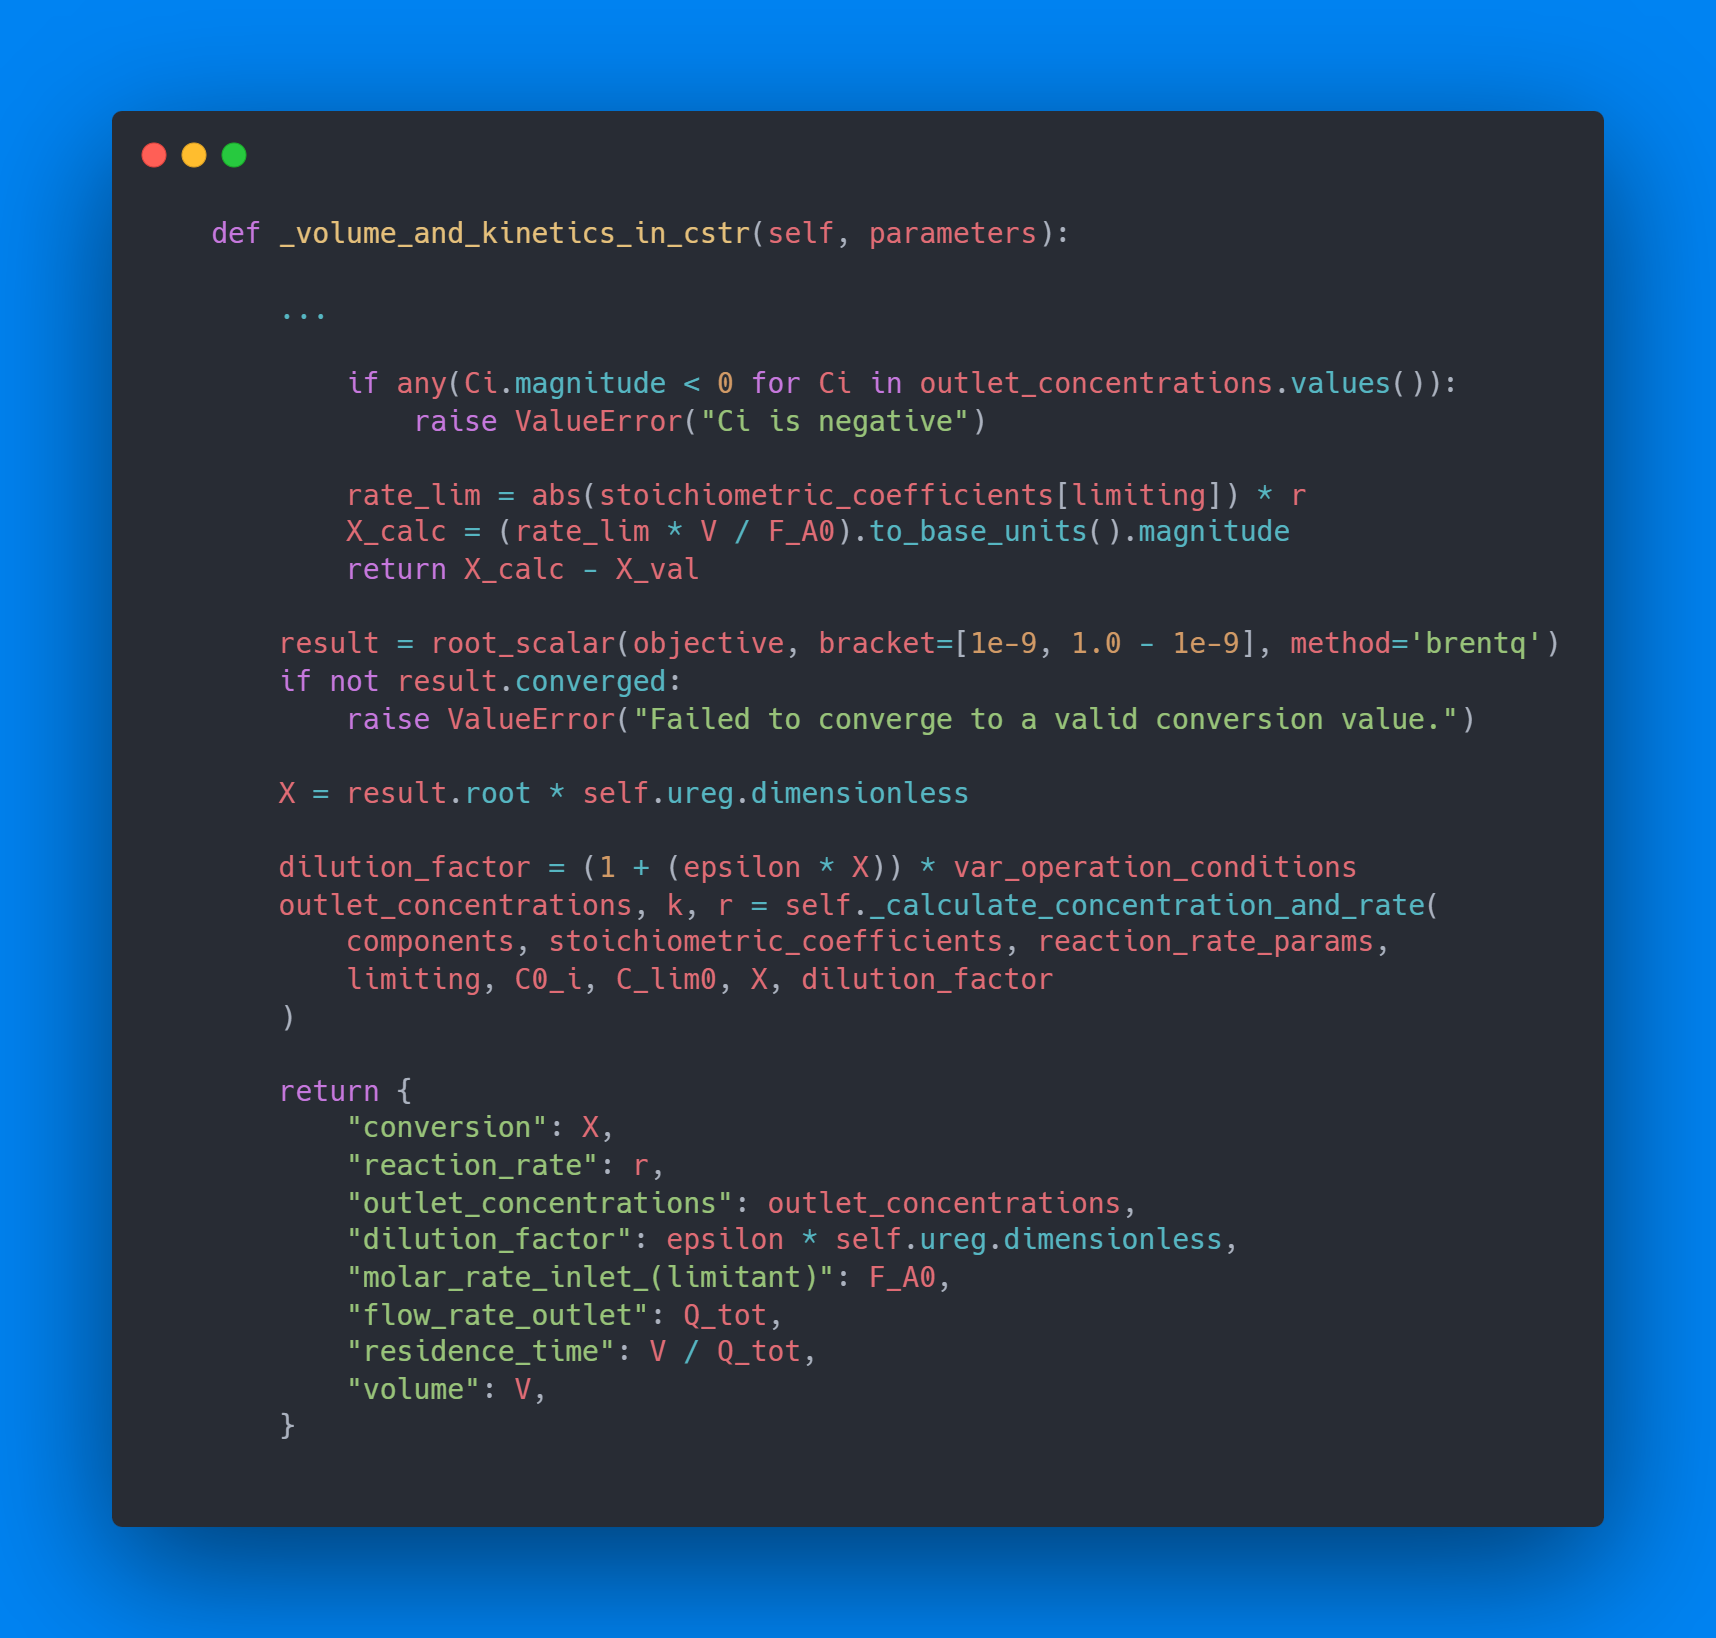
\includegraphics[width=\linewidth]{media/cap4_funcao_volume_and_kinetics_in_cstr_parte_dois.png}
    \fonte{Elaboração própria (2026).}
\end{figure}

\paragraph{Tempo de Residência e Cinética}

Conhecido o tempo de residência $\tau$, calcula-se inicialmente pela Equação \ref{eq:volume_calc}:
\begin{equation}
V = Q_{T} \cdot \tau
\label{eq:volume_calc}
\end{equation}
Em seguida, o problema se reduz ao caso anterior: aplica-se a mesma função objetivo $f ( X )$ da Equação \ref{eq:cstr_obj_function} e resolve-se numericamente para $X$, obtendo a conversão atingida no \textit{CSTR} com tempo de residência $\tau$ especificado.

\begin{figure}[H]
    \centering
    \caption{Código da função \textit{\_residence\_time\_and\_kinetics\_in\_cstr()} – Parte 1/2}
    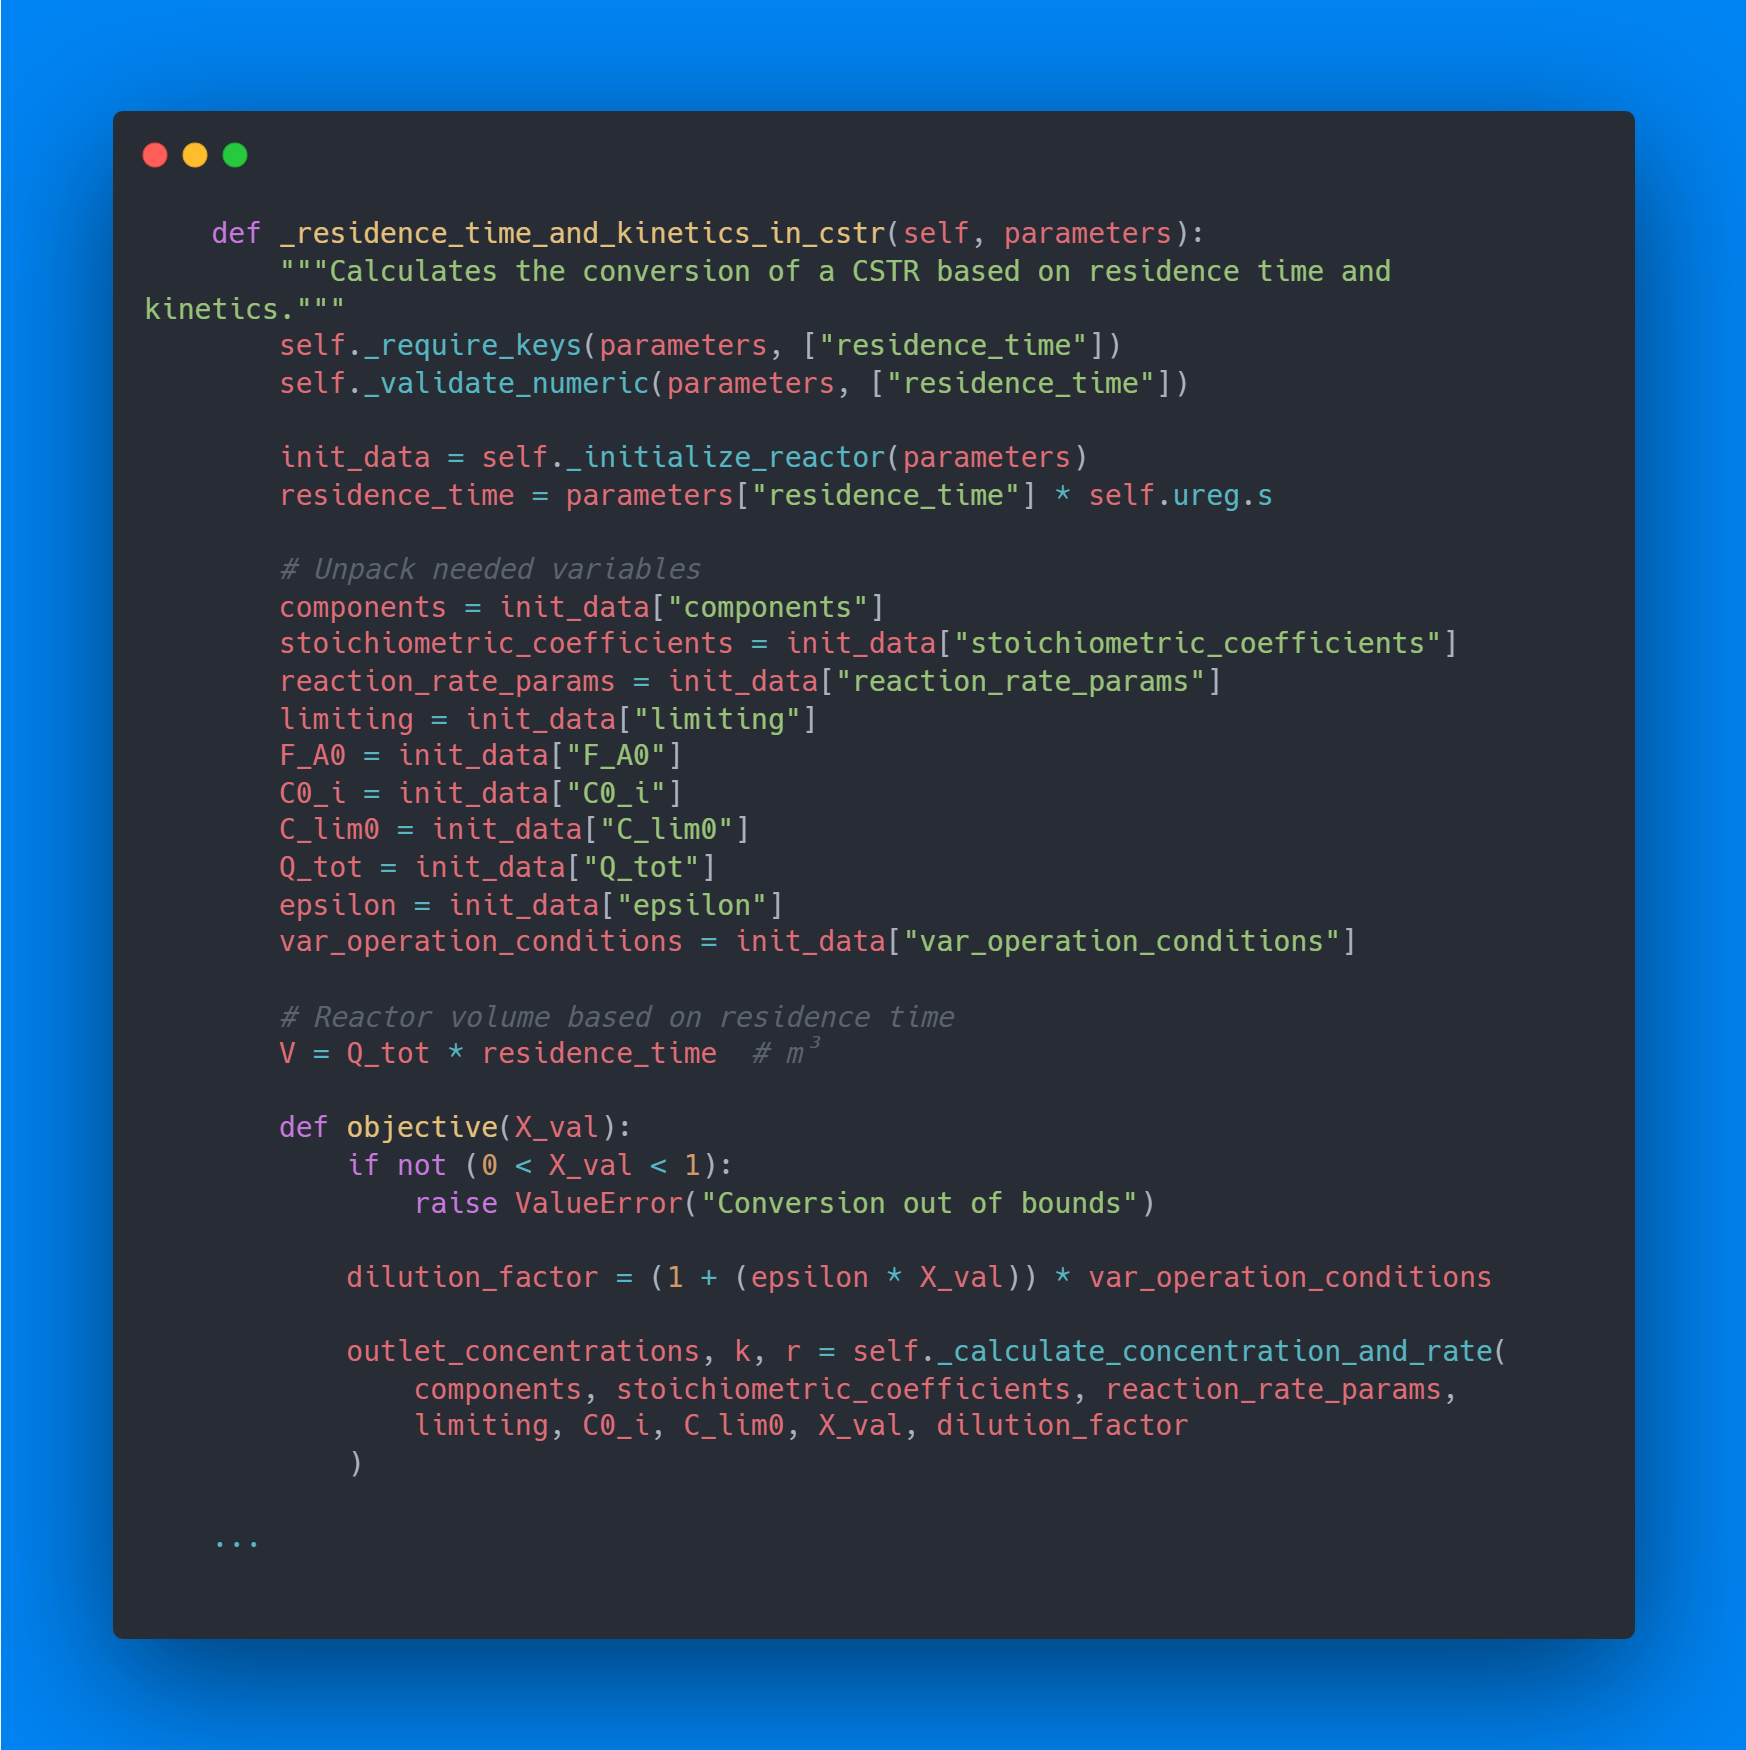
\includegraphics[width=\linewidth]{media/cap4_funcao_residence_time_and_kinetics_in_cstr_parte_um.png}
    \fonte{Elaboração própria (2026).}
\end{figure}

\begin{figure}[H]
    \centering
    \caption{Código da função \textit{\_residence\_time\_and\_kinetics\_in\_cstr()} – Parte 2/2}
    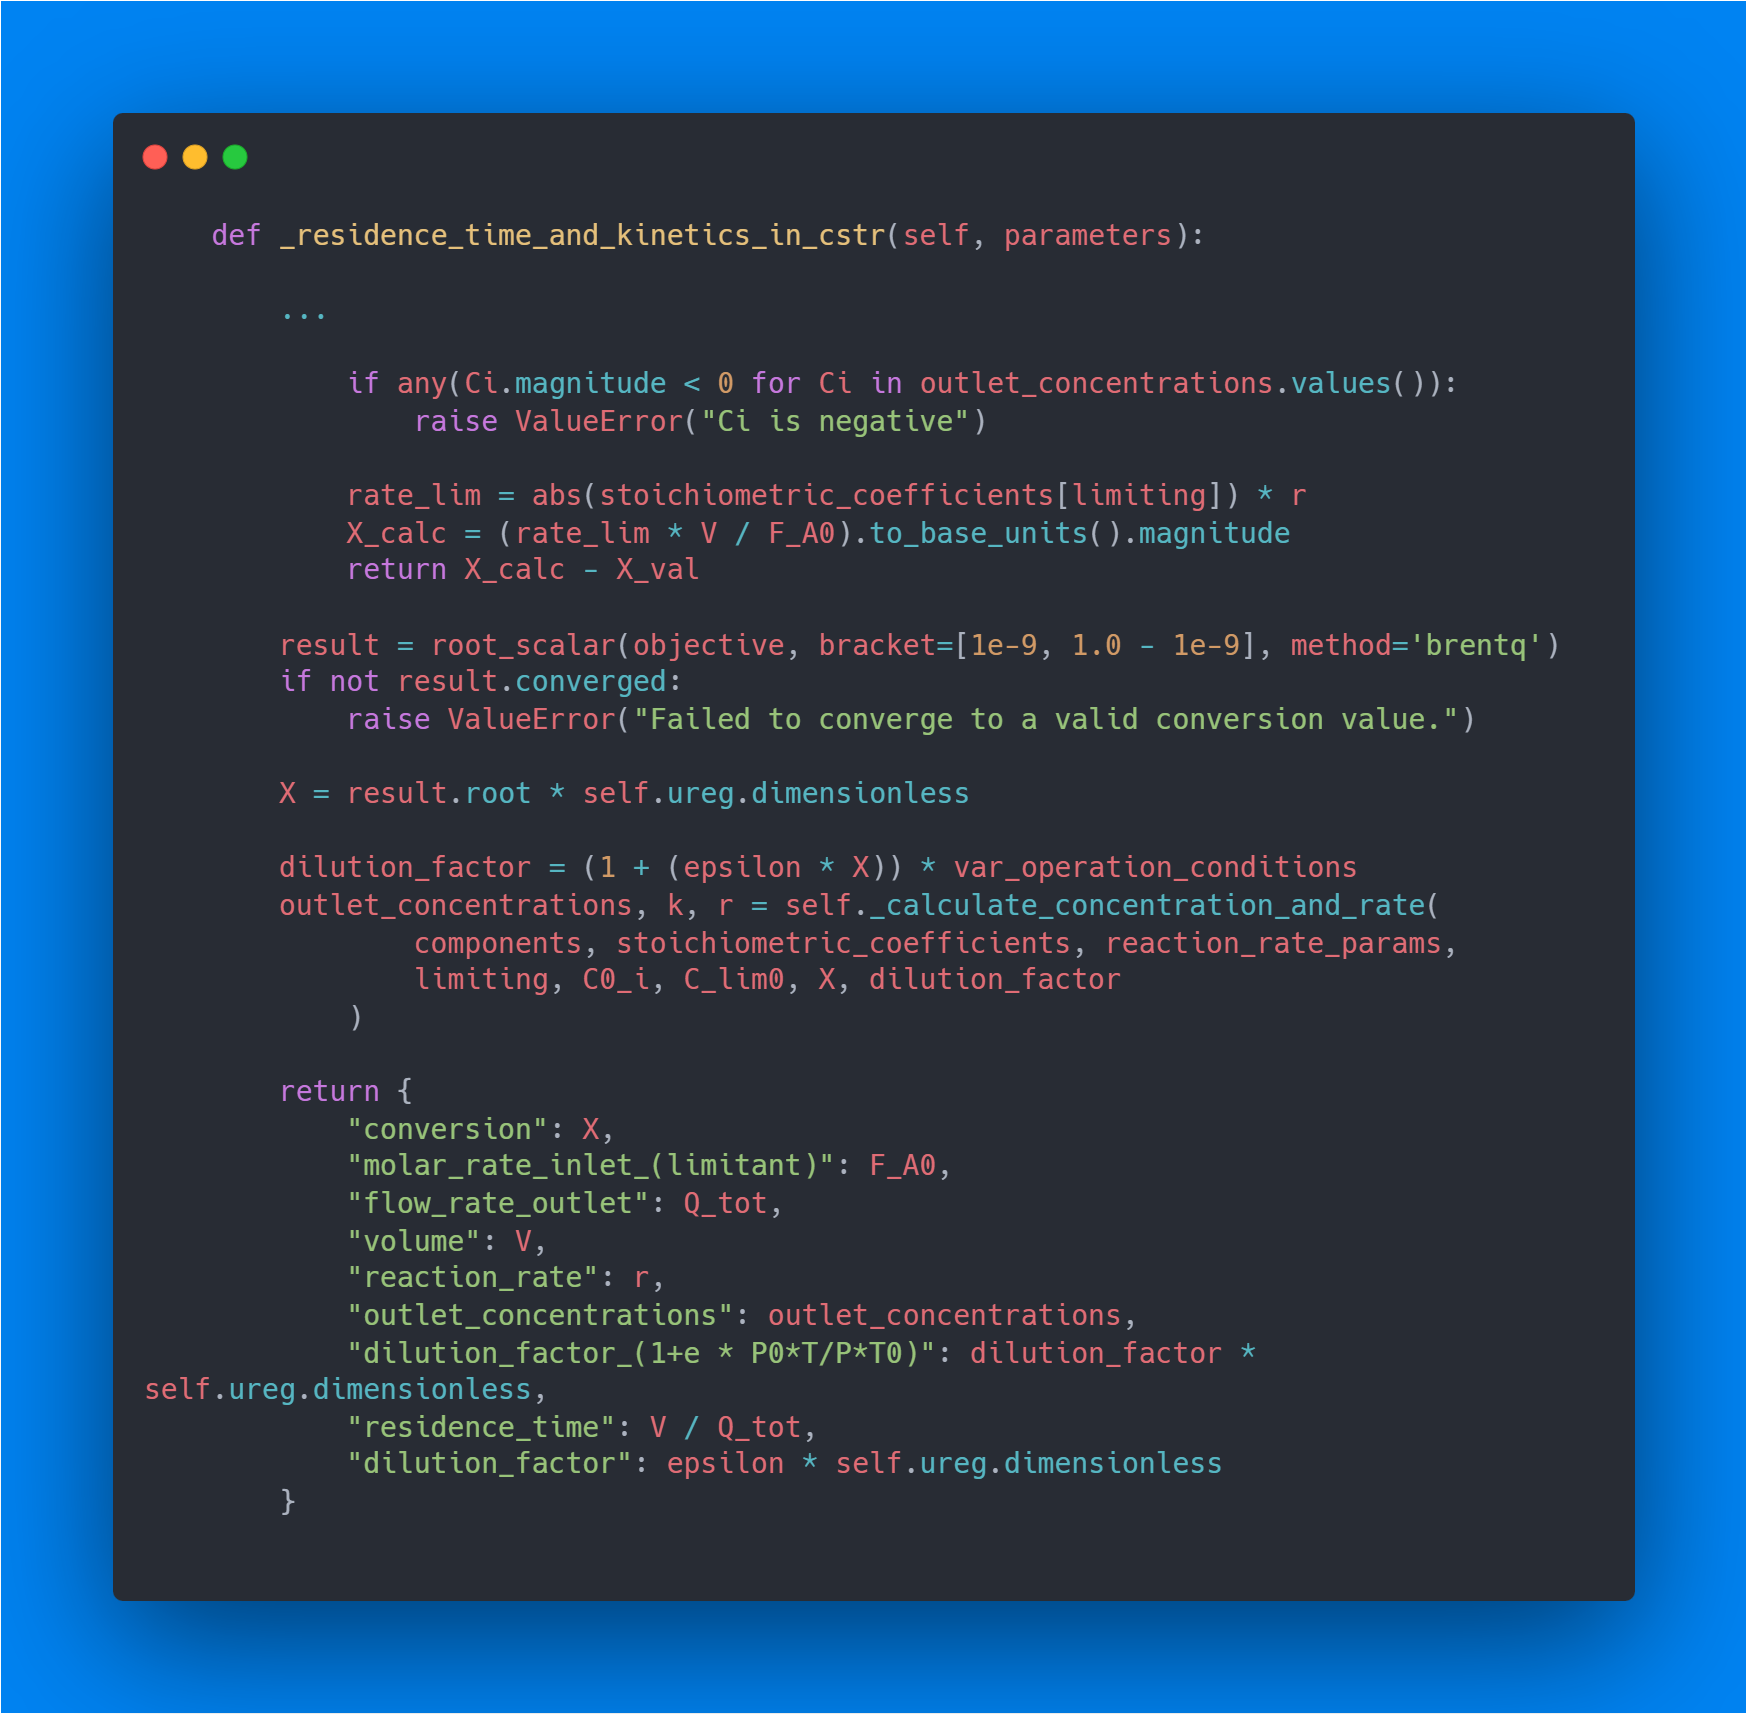
\includegraphics[width=\linewidth]{media/cap4_funcao_residence_time_and_kinetics_in_cstr_parte_dois.png}
    \fonte{Elaboração própria (2026).}
\end{figure}
